\documentclass[12pt]{report}

\voffset=-1.65cm
\oddsidemargin=0.0cm
\textwidth = 485pt

\usepackage{framed}
\usepackage{graphics}
\usepackage{amsmath}
\usepackage{color}
\usepackage{amssymb}
\usepackage{multicol}
\usepackage[dvipsnames]{xcolor}
\usepackage{graphicx}
%---------------------------------------%
%opening
\title{MA4413 and MA4704}
\author{Introduction to Probability}

\begin{document}
\LARGE
\section{Dice Questions}
	%----------------------------------------------------------%
		%http://www.indiabix.com/aptitude/probability/

		Suppose a pair of fair dice is thrown. 
		\begin{itemize}
			\item[(a)] What is the probability of getting a sum of 9 from two throws of a dice
		\end{itemize}
		Find the probability that the sum is 10 or greater if
		\begin{itemize}
			\item[(b)] a 5 appears on the first die, 
			\item[(c)] a 5 appears on at least one of the dice.
		\end{itemize}
		
		
		
		%----------------------------------------------------------%
	Tickets numbered 1 to 20 are mixed up and then a ticket is drawn at random. What is the probability that the ticket drawn has a number which is a multiple of 3 or 5

%===================================================================== %
\chapter{Mathematical Fundamentals}
\section*{The factorial function}
The factorial function (symbol: !) just means to multiply a series of descending natural numbers. Examples:

\begin{itemize}
	\item $4! = 4 \times 3 \times 2 \times 1 = 24$
	\item $7! = 7 \times 6 \times 5 \times 4 \times 3 \times 2 \times 1 = 5,040$
	\item $1! = 1$
	\item $0! = 1 $
\end{itemize}
Importantly 
\[n! = n \times (n-1)!  = n \times (n-1) \times (n-2)! \]
For Example
\[6! = 6 \times 5!  = 6 \times 5 \times 4! \]

		%\begin{multicol}{2}
		\begin{itemize}
			\item ${6 \choose 2} = 15$
			\item ${5 \choose 2} = 10$  
			\item ${4 \choose 0} = 1$  
			\item ${4 \choose 3} = 4$  
		\end{itemize}
		%\end{multicol}
		
			\begin{itemize}
				\item factorials 
				\[ n! = (n)\times (n-1)\times(n-2) \times \ldots \times 1 \]
				\begin{itemize}
					\item $5! = 5 \times 4 \times 3 \times 2 \times 1 = 120 $
					\item $3! = 3 \times 2 \times 1$
				\end{itemize}
				\item Zero factorial
				\[ 0! =  1 \]
			\end{itemize}
	
	\begin{itemize}
		\item[9B.1] Permutation
		
		\[ {n \choose r} = \frac{n!}{(n-r)! r!} \]
		
		
		\[ {6 \choose 3} = \frac{6!}{(6-3)! 3!} = \frac{6!}{3! \times 3!}\]
		
		
		\[ \frac{6!}{3! \times 3!} = \frac{6 \times 5 \times 4 \times 3!}{3! \times 3!} = \frac{120}{6} = 120\]
	\end{itemize}
	
	%\begin{multicol}{2}
	\begin{itemize}
		\item ${6 \choose 2} = 15$
		\item ${5 \choose 2} = 10$  
		\item ${4 \choose 0} = 1$  
		\item ${4 \choose 3} = 4$  
	\end{itemize}
	%\end{multicol}
	
%========================================================= %		
		
		\section{Counting Problems}
		\large
		\begin{itemize}
			\item Permutations where repetition is allowed: 
			\[ n! \]
			\item Permutations where repetition is not allowed
			\[ \frac{n!}{(n-k)!} \]
		\end{itemize}
		
		
		% http://www.mathsisfun.com/combinatorics/combinations-permutations.html
		
%%- \frametitle{Factorials Numbers}

A factorial is a positive whole number, based on a number $n$ , and which is written as $``n!"$. The factorial $n!$ is defined as follows:

\[n!  =n \times (n-1) \times (n-2) \times \ldots \times 2 \times 1 \]

Remark $n!  =n \times (n-1)!$\\ \bigskip

\textbf{ Example: }

\begin{itemize}
	\item $3!  = 3 \times 2  \times 1 = 6 $
	
	\item $4!  = 4 \times 3! = 4 \times 3 \times 2 \times 1 = 24$
\end{itemize}
Remark $0! = 1$ not $0$.



%--------------------------------------------------------%
{\Large
	%%- \frametitle{Permutations and Combinations}
	
	
	Often we are concerned with computing the number of ways of selecting and arranging groups of items. \begin{itemize} \item  A \textbf{\emph{combination}} describes the selection of items from a larger group of items.  \item A \textbf{\emph{permutation}} is a combination that is arranged in a particular way.
	\end{itemize}
	
	\bigskip
	\begin{itemize}
		\item Suppose we have items A,B,C and D to choose two items from.
		\item AB is one possible selection, BD is another. AB and BD are both combinations.
		\item More importantly, AB is one combination, for which there are two distinct permutations: AB and BA.
	\end{itemize}
}

%--------------------------------------------------------%
{\Large
	%%- \frametitle{Combinations}
	
	\textbf{Combinations: }
	The number of ways of selecting $k$ objects from $n$ unique objects is:
	
	\[ ^n C_k = {n!  \over k! \times (n-k)!} \]
	
	In some texts, the notation for finding the number of possible combination is written
	
	\[ ^n C_k =  {n \choose k} \]
	
}

%--------------------------------------------------------%
{\Large
	%%- \frametitle{Example of Combinations}
	How many ways are there of selecting two items from possible 5?
	
	\[ ^5 C_2   \left( \mbox{ also }  {5 \choose 2}  \right) =  {5!  \over 2! \times 3!} =  {5 \times 4 \times 3!  \over 2 \times 1 \times 3!} = 10  \]
	
	\bigskip
	Discuss how combinations can be used to compute the number of rugby matches for each group in the Rugby World Cup.
	
}
%--------------------------------------------------------%
{\Large
	%%- \frametitle{The Permutation Formula}
	The number of different permutations of r items from n unique items is written as $^n P_k$
	
	
	\[ ^n P_k = \frac{n!}{(n-k)!}\]
}

%--------------------------------------------------------%
{\Large
	%%- \frametitle{Permutations}
	\textbf{Example:}
	How many ways are there of arranging 3 different jobs, between 5 workers, where each worker can only do one job?
	
	
	\[ ^5 P_3 = \frac{5!}{(5-3)!}  = {5! \over 2!} = 60\]
	
}



%--------------------------------------------------------%
{\Large
	%%- \frametitle{Example of Combinations}
	
	A committee of 4 must be chosen from 3 females and 4 males.
	
	\begin{itemize}
		\item In how many ways can the committee be chosen.
		\item In how many cans 2 males and 2 females be chosen.
		\item Compute the probability of a committee of 2 males and 2 females are chosen.
		\item Compute the probability of at least two females.
	\end{itemize}
}

%--------------------------------------------------------%
{\Large
	%%- \frametitle{Example of Combinations}
	
	\textbf{Part 1}
	
	We need to choose 4 people from 7:
	
	This can be done in
	
	\[
	^7 C_4  = {7!  \over 4! \times 3!} =  {7 \times 6 \times 5 \times 4!  \over 4! \times 3!} = 35 \mbox{ ways.}
	\]
	
	
	\textbf{Part 2}
	
	With 4 men to choose from, 2 men can be selected in \[
	^4 C_2  = {4!  \over 2! \times 2!} =  {4 \times 3 \times 2!  \over 2! \times 2!} = 6\mbox{ ways.}
	\]
	
	Similarly 2 women can be selected from 3 in
	\[
	^3 C_2  = {3!  \over 2! \times1!} =  {3 \times 2!  \over 2! \times 1!} = 3\mbox{ ways.}
	\]
	
}

%============================================================== %
When implementing combination calculations in \texttt{R}, we use the \texttt{choose()} function.
\begin{framed}	
	\begin{verbatim}
	> choose(5,0)
	[1] 1
	> choose(5,1)
	[1] 5
	> choose(5,2)
	[1] 10
	> choose(5,3)
	[1] 10
	> choose(5,4)
	[1] 5
	> choose(5,5)
	[1] 1
	\end{verbatim}
\end{framed}
	
	%% ----------------------------------%%
	%--------------------------------------------------------%
	{\Large
		%%- \frametitle{Example of Combinations}
		
		\textbf{Part 2}
		
		Thus a committee of 2 men and 2 women can be selected in $ 6 \times 3  = 18 $ ways.\\
		\bigskip
		\textbf{Part 3}
		
		The probability of two men and two women on a committee is
		\[ {\mbox{Number of ways of selecting 2 men and 2 women} \over \mbox{Number of ways of selecting 4 from 7}} = {18 \over 35 }\]
		
	}
	%--------------------------------------------------------%
	{\Large
		%%- \frametitle{Example of Combinations}
		
		\textbf{Part 4}
		\begin{itemize}
			\item The probability of at least two females is the probability of 2 females or 3 females being selected.
			\item We can use the addition rule, noting that these are two mutually exclusive events.
			\item From before we know that probability of 2 females being selected is 18/35.
		\end{itemize}
		
	}
	%--------------------------------------------------------%
	{\Large
		%%- \frametitle{Example of Combinations}
		
		\textbf{Part 4}
		\begin{itemize}
			\item We have to compute the number of ways of selecting 1 male from 4 (4 ways) and the number of ways of selecting three females from 2 ( only 1 way)
			\item The probability of selecting three females is therefore ${4 \times 1 \over 35} = 4/35$
			\item So using the addition rule
			\[ Pr(\mbox{ at least 2 females }) = Pr(\mbox{ 2 females }) + Pr(\mbox{ 3 females }) \]
			\[ Pr(\mbox{ at least 2 females })  = 18/35 + 4/35 = 22/35 \]
		\end{itemize}
		
	}
	
	
	
	%--------------------------------------------------------%
	\section{ Combinations and Permutations }
	
	%--------------------------------------------------------%
	{\Large
		%%- \frametitle{Factorials Numbers}
		
		A factorial is a positive whole number, based on a number $n$ , and which is written as $``n!"$. The factorial $n!$ is defined as follows:
		
		\[n!  =n \times (n-1) \times (n-2) \times \ldots \times 2 \times 1 \]
		
		Remark $n!  =n \times (n-1)!$\\ \bigskip
		
		\textbf{ Example: }
		
		\begin{itemize}
			\item $3!  = 3 \times 2  \times 1 = 6 $
			
			\item $4!  = 4 \times 3! = 4 \times 3 \times 2 \times 1 = 24$
		\end{itemize}
		Remark $0! = 1$ not $0$.
		
		
	}
	
	%--------------------------------------------------------%
	{\Large
		%%- \frametitle{Permutations and Combinations}
		
		
		Often we are concerned with computing the number of ways of selecting and arranging groups of items. \begin{itemize} \item  A \textbf{\emph{combination}} describes the selection of items from a larger group of items.  \item A \textbf{\emph{permutation}} is a combination that is arranged in a particular way.
		\end{itemize}
		
		\bigskip
		\begin{itemize}
			\item Suppose we have items A,B,C and D to choose two items from.
			\item AB is one possible selection, BD is another. AB and BD are both combinations.
			\item More importantly, AB is one combination, for which there are two distinct permutations: AB and BA.
		\end{itemize}
	}
	
	%--------------------------------------------------------%
	{\Large
		%%- \frametitle{Combinations}
		
		\textbf{Combinations: }
		The number of ways of selecting $k$ objects from $n$ unique objects is:
		
		\[ ^n C_k = {n!  \over k! \times (n-k)!} \]
		
		In some texts, the notation for finding the number of possible combination is written
		
		\[ ^n C_k =  {n \choose k} \]
		
	}
	
	%--------------------------------------------------------%
	{\Large
		%%- \frametitle{Example of Combinations}
		How many ways are there of selecting two items from possible 5?
		
		\[ ^5 C_2   \left( \mbox{ also }  {5 \choose 2}  \right) =  {5!  \over 2! \times 3!} =  {5 \times 4 \times 3!  \over 2 \times 1 \times 3!} = 10  \]
		
		\bigskip
		Discuss how combinations can be used to compute the number of rugby matches for each group in the Rugby World Cup.
		
	}
	%--------------------------------------------------------%
	{\Large
		%%- \frametitle{The Permutation Formula}
		The number of different permutations of r items from n unique items is written as $^n P_k$
		
		
		\[ ^n P_k = \frac{n!}{(n-k)!}\]
	}
	
	%--------------------------------------------------------%
	{\Large
		%%- \frametitle{Permutations}
		\textbf{Example:}
		How many ways are there of arranging 3 different jobs, between 5 workers, where each worker can only do one job?
		
		
		\[ ^5 P_3 = \frac{5!}{(5-3)!}  = {5! \over 2!} = 60\]
		
	}
	
	
	
	%--------------------------------------------------------%
	{\Large
		%%- \frametitle{Example of Combinations}
		
		A committee of 4 must be chosen from 3 females and 4 males.
		
		\begin{itemize}
			\item In how many ways can the committee be chosen.
			\item In how many cans 2 males and 2 females be chosen.
			\item Compute the probability of a committee of 2 males and 2 females are chosen.
			\item Compute the probability of at least two females.
		\end{itemize}
	}
	
	%--------------------------------------------------------%
	{\Large
		%%- \frametitle{Example of Combinations}
		
		\textbf{Part 1}
		
		We need to choose 4 people from 7:
		
		This can be done in
		
		\[
		^7 C_4  = {7!  \over 4! \times 3!} =  {7 \times 6 \times 5 \times 4!  \over 4! \times 3!} = 35 \mbox{ ways.}
		\]
		
		
		\textbf{Part 2}
		
		With 4 men to choose from, 2 men can be selected in \[
		^4 C_2  = {4!  \over 2! \times 2!} =  {4 \times 3 \times 2!  \over 2! \times 2!} = 6\mbox{ ways.}
		\]
		
		Similarly 2 women can be selected from 3 in
		\[
		^3 C_2  = {3!  \over 2! \times1!} =  {3 \times 2!  \over 2! \times 1!} = 3\mbox{ ways.}
		\]
		
	}
	MA4704 Tutorial Sheet 2. 


Question 1

A doctor treating a patient issues a prescription for antibiotics and provides for two repeat prescriptions. The probability that the infection will be cleared by the first prescription is p1 =0.6. 
The probability that successive treatments are successful, given that previous prescriptions were not successful are p2 = 0.5, p3 = 0.4. Calculate the probability that  
   
1.	the patient is still infected after the third prescription
2.	the patient is cured by the second prescription.
3.	the patient is cured by the second prescription, given that the patient is eventually cured.


Question 2
A driver passes through 3 traffic lights. The chance he/she will stop at the first is 1/2 , at the second 1/3 and at the third ¼ independently of what happens at any of the other lights. 

What is the probability that
4.	the driver makes the whole journey without being stopped at any of the lights
5.	the driver is only stopped at the first and third lights
6.	the driver is stopped at just one set of lights.
7.	the driver stopped at the second set of lights, given he/she stopped at one set of lights.

Question 3
The masses of 30 human males and 30 arabian stallions were observed. Their masses (in lbs) are given below

Humans
106, 120, 130, 138, 145, 151, 156, 161, 166, 171
176, 180, 185, 189, 194, 198, 203, 208, 212, 217
223, 228, 234, 240, 247, 255, 264, 276, 290, 313



Stallions
808, 824, 835, 843, 851, 857, 862, 868, 872, 877
881, 886, 890, 894, 898, 902, 906, 910, 914, 919
923, 928, 932, 938, 943, 949, 957, 965, 976, 992


a)	Draw histograms for these samples and compare them with respect to shape, centrality and relative dispersion. 
b)	Calculate the medians of these samples (from the raw data).




Question 4

 

Question 5
The following data give the marks of 10 students in a test (out of 20 marks). Calculate
i) the median    ii) the mean     iii) the range    iv) the standard deviation v) The Inter-Quartile Range

12, 17, 7, 11, 18, 6, 14, 15, 11, 9.


%======================================================== %
		%%- \frametitle{Using \texttt{R}}
		When implementing combination calculations in \texttt{R}, we use the \texttt{choose()} function.
		
		\begin{verbatim}
		> choose(5,0)
		[1] 1
		> choose(5,1)
		[1] 5
		> choose(5,2)
		[1] 10
		> choose(5,3)
		[1] 10
		> choose(5,4)
		[1] 5
		> choose(5,5)
		[1] 1
		\end{verbatim}
		
		%% ----------------------------------%%
		%--------------------------------------------------------%
		{\Large
			%%- \frametitle{Example of Combinations}
			
			\textbf{Part 2}
			
			Thus a committee of 2 men and 2 women can be selected in $ 6 \times 3  = 18 $ ways.\\
			\bigskip
			\textbf{Part 3}
			
			The probability of two men and two women on a committee is
			\[ {\mbox{Number of ways of selecting 2 men and 2 women} \over \mbox{Number of ways of selecting 4 from 7}} = {18 \over 35 }\]
			
		}
		%--------------------------------------------------------%
		{\Large
			%%- \frametitle{Example of Combinations}
			
			\textbf{Part 4}
			\begin{itemize}
				\item The probability of at least two females is the probability of 2 females or 3 females being selected.
				\item We can use the addition rule, noting that these are two mutually exclusive events.
				\item From before we know that probability of 2 females being selected is 18/35.
			\end{itemize}
			
		}
		%--------------------------------------------------------%
		{\Large

			\begin{itemize}
				\item We have to compute the number of ways of selecting 1 male from 4 (4 ways) and the number of ways of selecting three females from 2 ( only 1 way)
				\item The probability of selecting three females is therefore ${4 \times 1 \over 35} = 4/35$
				\item So using the addition rule
				\[ Pr(\mbox{ at least 2 females }) = Pr(\mbox{ 2 females }) + Pr(\mbox{ 3 females }) \]
				\[ Pr(\mbox{ at least 2 females })  = 18/35 + 4/35 = 22/35 \]
			\end{itemize}
			
		}
%=========================================================== %
\newpage		
		\section*{Combinations and Permutations }
		\section*{Combinations}
		In mathematical terms, a combination is an subset of items from a larger set such that the order of the items does not matter.
		
		\subsection{Permutations}
		\Large
		\begin{itemize}
			\item The notion of permutation relates to the act of permuting (rearranging) objects or values. 
			\item Informally, a permutation of a set of objects is an arrangement of those objects into a particular order. 
			
			\item For example, there are six permutations of the set $\{1,2,3\}$, namely (1,2,3), (1,3,2), (2,1,3), (2,3,1), (3,1,2), and (3,2,1). 
			\item As another example, an anagram of a word is a permutation of its letters. 
			
		\end{itemize}
		
If the probability of C is $70 \%$ then the probability of $C^{\prime}$ is $30\%$		

%================================================================ %
\section*{Combinations}

\subsection*{Formula}
\[ \binom nk  = \frac{n!}{k!(n-k)!} = \frac{n(n-1)\ldots(n-k+1)}{k(k-1)\dots 1},\]
which can be written using factorials as  whenever $k\leq n$

\subsection*{Example 1}

\[ \binom 5 2  = \frac{5!}{2!\;(5-2)!} = \frac{5.4.3!}{2! .3!} = \frac{5.4}{2.1} = 10\]

\subsection*{Example 2}

\[ \binom 5 0   = \frac{5!}{0!\;(5-0)!} = \frac{5!}{0! .5!} = \frac{5!}{2!} = 1\]
Recall $0! =1$
%-----------------------------------------------------%
\section{Urn Questions}	

%----------------------------------------------------------%
\bigskip 
\textbf{Urn Questions}
%----------------------------------------------------------%
%page66
Suppose an urn contains seven white, four black and three red beads. Three beads are picked at random without replacement.
Find the probability that all three beads are the different in colour.
at least two beads are the same colour.
\begin{itemize}	
	%----------------------------------------------------------%
	\item A bag contains 2 red, 3 green and 2 blue balls. Two balls are drawn at random. What is the probability that none of the balls drawn is blue?
	
	
	
	%----------------------------------------------------------%
	\bigskip 
	\textbf{Independent Events}
	%----------------------------------------------------------%
	\item Competitors A and B fire at their respective targets. The probability that A hits a target is 1/3 and the probability that B hits a target is 1/5. Find the probability that:
	\begin{itemize}
		\item[i.] (2 marks) A does not hit the target,
		\item[ii.](2 marks)  both hit their respective targets,
		\item[iii.](2 marks)  only one of them hits a target,
		\item[iv.](2 marks) neither A nor B hit their targets.
	\end{itemize}
	%---------------------------------------------------------- %
	
	% Page 32
	\item Four Students work independently on a mathematical problem. The probability that the four students have of solving the problem are as follows:
	%----------------------------------------------------------%
	\item An IT consultant is responsible for three software engineering projects X, Y and Z.
	He knows that the probability of completing project X in time is 0.99, for project Y this probability is 0.95
	and for project Z it is 0.80.
	
	\begin{itemize}
		\item[a] What assumption do you need to make in order to calculate the probability
		of completing all three projects in time, from the information given?
		\item[b] Calculate the probability of completing all three projects in time.
		\item[c] Calculate the probability that only projects X and Y will be completed on time.
	\end{itemize}
	
	\item A doctor treating a patient issues a prescription for antibiotics and provides for two repeat prescriptions. The probability that the infection will be cleared by the first prescription is $p_1$ =0.6.
	The probability that successive treatments are successful, given that previous prescriptions were not successful are $p_2$ = 0.5, $p_3$ = 0.4. Calculate the probability that:
	
	\begin{itemize}
		\item[a] a patient will require the third prescription,
		\item[b] the patient is still infected after the third prescription,
		\item[c] the patient is cured by the second prescription, given that the patient is eventually cured.
	\end{itemize}
	
	%Page 29
	\item Two people look at the letters in the word discovery. Independently of each other, each person writes down two of the letters from the word discovery.
	What is the probability that
	\begin{itemize}
		\item[(i)] One person writes down two vowels and the other person 
		\item[(ii)]
	\end{itemize}
	%----------------------------------------------------------%
	%Page 73
	
	\item Three cards are drawn, one after the other, without replacement, from a pack of 52 playing cards.
	Find the probability that the
	
	
	
	
	
	\item
	On completion of a programming project, three programmers from a team submit a collection of subroutines to an acceptance group. \\
	\\
	The following table shows the percentage of subroutines each programmer submitted and the probability that a subroutine submitted by each programmer will pass the certification test based on historical data.
	
	\begin{center}
		\begin{tabular}{|l|c|c|c|}
			\hline
			Programmer &	A	&B	& C	\\\hline
			Proportion of subroutines submitted&	0.40	&0.35	&0.25	\\ \hline
			Probability of acceptance	&0.75	&0.95	&0.85\\
			
			\hline
		\end{tabular}
	\end{center}
\end{itemize}
\begin{itemize}
	\item[i.] (3 marks) What is the proportion of subroutines that pass the acceptance test?
	\item[ii.](3 marks)  After the acceptance tests are completed, one of the subroutines is selected at random and found to have passed the test. What is the probability that it was written by Programmer A?
\end{itemize}

%============================================================================================ %
\newpage
		\section{Permutations}
		\Large
		\begin{itemize}
			\item Permutations where repetition is allowed: 
			\[ n! \]
			\item Permutations where repetition is not allowed
			\[ \frac{n!}{(n-k)!} \]
		\end{itemize}
\textbf{\;\;\;Choose Operator}
%----------------------------------------------------------%
\begin{itemize}
	%----------------------------------------------------------%
	
	
	\item[1] Choose Operator
	\[ {n \choose k} = \frac{n!}{k! \times (n-k)!} \]
	Evaluate the following:
	\begin{multicols}{3}
		\begin{enumerate}
			\item[1] ${5 \choose 2}$
			\item[2] ${5 \choose 0}$
			\item[3] ${6 \choose 3}$
			\item[4] ${6 \choose 6}$
			\item[5] ${10 \choose 1}$
			\item[6] ${10 \choose 9}$
		\end{enumerate}        
	\end{multicols}
	%----------------------------------------------------------%
	%Page 29
	\item[2] In how many ways can a group of four people be selected from three men and four women?
	In how many of these groups are there more women than men?
	%----------------------------------------------------------%
	%PAGE 66
	\item[3] In how many ways can a group of five be selected from ten people
	How many groups can be selected if two particular people from the ten can not be selected in the same group?\\
	\\
	\textbf{Counting Sets using Venn Diagrams}
	\item[4] 
	%http://www.mathsireland.com/LCHGeneralNotes/PermCombProb/5_5_Prob_MultAnd/Q_5_5_Prob_MultAnd.html
	The Venn Diagram shows the number of elements in each subset of set $S$.
	If $P(A) = 3/10$ and $P(B) = 1/2$, find the values of $x$ and $y$
	
	%Page 27
	\item[5] How many different four digit numners greater than 5000 can be formed from the digits \textbf{2,4,5,8,9} if each digit can only be used once in any given number. How many of these numbers are odd?
\end{itemize}
%============================================================= %
	\section*{Type of Permutations}
		There are two types of permutation:
		\begin{enumerate}
			\item Repetition is Allowed: such as the lock above. It could be "333".
			\item No Repetition: for example the first three people in a running race. You can't be first and second.
		\end{enumerate}
		
		\subsection*{Summary}
		\begin{itemize}
			\item If the order doesn't matter, it is a Combination.
			\item If the order does matter it is a Permutation.
		\end{itemize}
		%-------------------------------------%
		
		\subsection{Permutations}
	
		How many anagrams (permutations of the letters) are there of the following words
		\begin{enumerate}
			\item ANSWER
			\item PERMUTE
			\item ANAGRAM
			\item LITTLE
		\end{enumerate}
		
		
		\textbf{Part 1 : ANSWER}\\
		Examples:
		\begin{center}
			ASNWRE,\;
			SANERW,\;
			REWSAN,\;...
		\end{center}
		
		Since ANSWER has 6 distinct letters, the number of permutations (anagrams) is
		\LARGE
		\[6! = 6\times 5 \times 4 \times 3 \times 2\times 1 = \boldsymbol{720} \]
		
		\vspace{-0.3cm}
		\textbf{Part 2 : PERMUTE}\\
		\begin{itemize}
			\item The word PERMUTE has 7 letters, but only 6 different letters. 
			\item There are 7! ways to arrange 7 letters.
			\item However, interchanging the two Es does not result in a new permutation. There would be two identical anagrams.
		\end{itemize}
		
		\begin{center}
			P\textcolor{red}{E}RMUT\textcolor{blue}{E}, \; MUT\textcolor{red}{E}P\textcolor{blue}{E}R, \; P\textcolor{red}{E}T\textcolor{blue}{E}MUR,\; ..\\
			P\textcolor{blue}{E}RMUT\textcolor{red}{E}, \; MUT\textcolor{blue}{E}P\textcolor{red}{E}R, \; P\textcolor{blue}{E}T\textcolor{red}{E}MUR,\; ..
		\end{center}
		

		\textbf{Part 2 : PERMUTE}\\
		\begin{itemize}
			\item The number of permutations (anagrams) is half of 7! .
			\LARGE
			\[\frac{7!}{2} =  \frac{5040}{2} = \boldsymbol{2520} \]
		\end{itemize}
		
		
		\textbf{Part 3 : ANAGRAM}\\
		\begin{itemize}
			\item The word ANAGRAM has 7 letters, but there are three As.
			\item From before, there are 7! ways to arrange 7 letters.
			\item How many new permutations are found by re-arranging the As?
		\end{itemize}
		\LARGE
		\begin{itemize}
		\item	\textcolor{red}{A}N\textcolor{blue}{A}GR\textcolor{purple}{A}M 
	\item		\textcolor{red}{A}N\textcolor{purple}{A}GR\textcolor{blue}{A}M 
	\item 		\textcolor{blue}{A}N\textcolor{red}{A}GR\textcolor{purple}{A}M  \\
	\item		\textcolor{purple}{A}N\textcolor{red}{A}GR\textcolor{blue}{A}M 
		\item	\textcolor{blue}{A}N\textcolor{purple}{A}GR\textcolor{red}{A}M 
	\item		\textcolor{purple}{A}N\textcolor{blue}{A}GR\textcolor{red}{A}M 
		\end{itemize}

		\vspace{-0.1cm}
		\textbf{Part 3 : ANAGRAM}\\
		\begin{itemize}
			\item We divide 7! by 3! to account for the identical anagrams.
			\LARGE
			\[\frac{7!}{3!} =  \frac{5040}{6} = \boldsymbol{840} \]
		\end{itemize}
		
		%-------------------------------------%
		
		\subsection{Permutations}
		\Large
		\vspace{-2.3cm}
		\textbf{Part 2 : PERMUTE}\\
		\begin{itemize}
			\item We re-express the answer from part 2 as follows:
			\LARGE
			\[\frac{7!}{2!} =  \frac{5040}{2} = \boldsymbol{2520} \]
		\end{itemize}
		
		\textbf{Part 4 : LITTLE}\\
		\begin{itemize}
			\item The word LITTLE has 6 letters, but there are two Ls and two Ts.
			\item From before, there are 6! ways to arrange 6 letters.
			\item Again, interchanging the two Ls and Ts does not result in a new permutation. 
			\LARGE
			\[\frac{6!}{2!\times 2!} =  \frac{720}{4} = \boldsymbol{180} \]
		\end{itemize}
		
		%------------------------------------------------------ %
		
		\subsection{Permutations}
		\large
		\begin{itemize}
			\item In how many permutations are there of counting a subset of k elements, when there are $n$ elements in total.
			
			\item The number of permutations of a set of n elements is denoted n! (pronounced n factorial.)
		\end{itemize}
		
		%------------------------------------------------------ %
		
		\subsection{Permutation Formula}
		
		A formula for the number of possible permutations of k objects from a set of n. This is usually written $^nP_k$ .
		
		\bigskip
		\textbf{Formula:}	
		\[ ^nP_k = \frac{n!}{(n-k)!} =  n.(n-1).(n-2).\ldots(n-k+1) \]
		
		
		
		\textbf{Example:}\\	
		How many ways can 4 students from a group of 15 be lined up for a photograph?\\
		\bigskip
		%--------------- %
		\textbf{Answer:	}\\
		There are $^{15}P_4$ possible permutations of 4 students from a group of 15.
		\[ ^{15}P_4 = \frac{15!}{11!} = 15\times 14\times 13\times 12 = 32760 \]
		There are 32760 different lineups.
		
	
\section{Counting}
% 2007 Q8
Given S is the set of all 5 digit binary strings, E is the set of a 5 digit
binary strings beginning with a 1 and F is the set of all 5 digit binary strings ending
with two zeroes.
\begin{itemize}
	\item[(a)] Find the cardinality of S, E and F.
	\item[(b)] Draw a Venn diagram to show the relationship between the sets S, E and F.
	Show the relevant number of elements in each region of your diagram.
\end{itemize}
%-------------------------------------------------------------------------%
%-----------------------------------------------------%

{\LARGE
	%% \frametitle{Overview of Current Part of Course}
	Probability Distributions (Question 2 for End Of Year Exam)
	\begin{itemize}
		\item Discrete Probability Distributions
		\begin{itemize}
			\item Binomial Probability Distribution (Week 3)
			\item Geometric Probability Distribution (Week 3)
			\item Poisson Probability Distribution (Week 3/4)
		\end{itemize}
		
		\item Continuous Probability Distributions
		\begin{itemize}
			\item Exponential Probability Distribution (Week 4)
			\item Uniform Probability Distribution (Week 4)
			\item Normal Probability Distribution (Week 4/5)
		\end{itemize}
	\end{itemize}
}

%% ----------------------------------%%
%% \frametitle{Continuous Random variables}
\begin{itemize}
	\item Previously we have been studying discrete random variables, such as the Binomial and the Poisson random variables.
	\item Now we turn our attention to continuous random variables.
	\item Recall that a continuous random variable is one which takes an infinite number of possible values, rather than just a countable number of distinct values.
	\item Continuous random variables are usually measurements.
	\item Examples include height, weight, the amount of sugar in an orange, the time required to run a mile.
\end{itemize}
%% ----------------------------------%%
%------------------------------------------------------------------%
{\LARGE
	%% \frametitle{Exact Probabilities}
	\large
	\textbf{Remarks:} This is for continuous distributions only.
	\begin{itemize}
		\item The probability that a continuous random variable will take an exact value is infinitely small.
		We will usually treat it as if it was zero.
		\item
		When we write probabilities for continuous random variables in mathematical notation, we often retain the equality component (i.e. the "...or equal to..").\\
		For example, we would write expressions $P(X \leq 2)$ or $P(X \geq 5)$.
		\item
		Because the probability of an exact value is almost zero, these two expression are equivalent to $P(X < 2)$
		or $P(X > 5)$. \item Also, the complement of $P(X \geq k)$ can be written as $P(X \leq k)$.
	\end{itemize}
}
%----------------------------------------------------------------------------------------------------%
%% ----------------------------------%%
%% \frametitle{Functions and Definite integrals}
\begin{itemize}
	\item Integration is not part of the syllabus, and it is assumed that students are not familiar with how to compute definite integrals.
	\item However,  it is useful to know what the purpose of definite integrals are, because we will be using the results derived from definite integrals. \item It is assumed that students are familiar with functions.
\end{itemize}
%% ----------------------------------%%
%----------------------------------------------------------------------------------------------------%
%% ----------------------------------%%
%% \frametitle{Functions}

\vspace{-0.5cm}
\begin{figure}
	\centering
	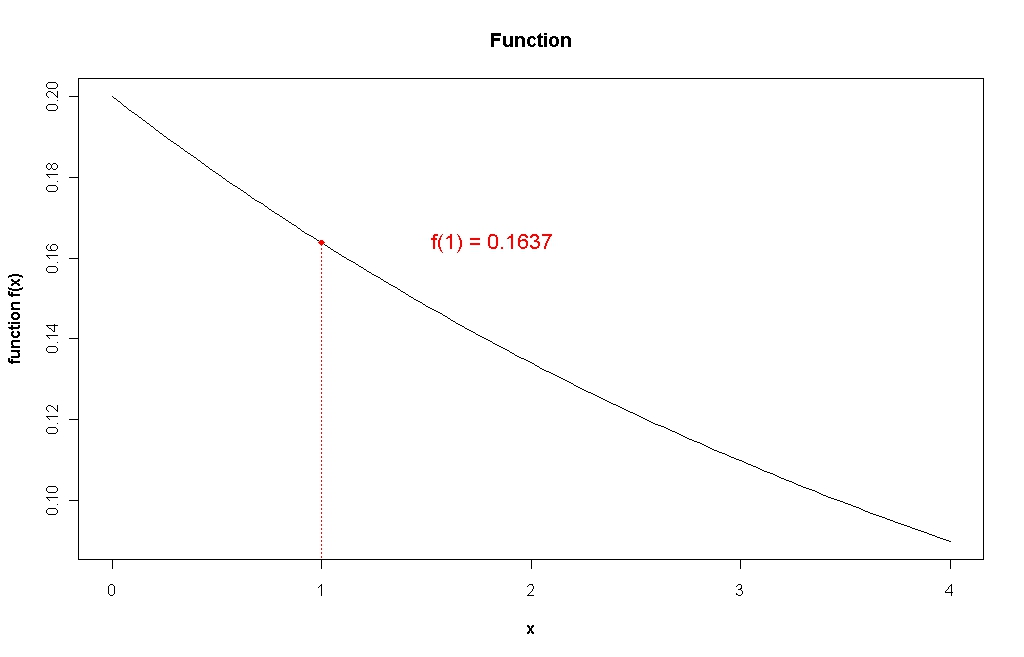
\includegraphics[width=0.7\linewidth]{images/6AFunction}
	\caption{}
	\label{fig:6AFunction}
\end{figure}


Some function $f(x)$ evaluated at $x=1$.
%% ----------------------------------%%
%----------------------------------------------------------------------------------------------------%
%% ----------------------------------%%
%% \frametitle{Definite Integral}

\vspace{-0.5cm}
\begin{center}
	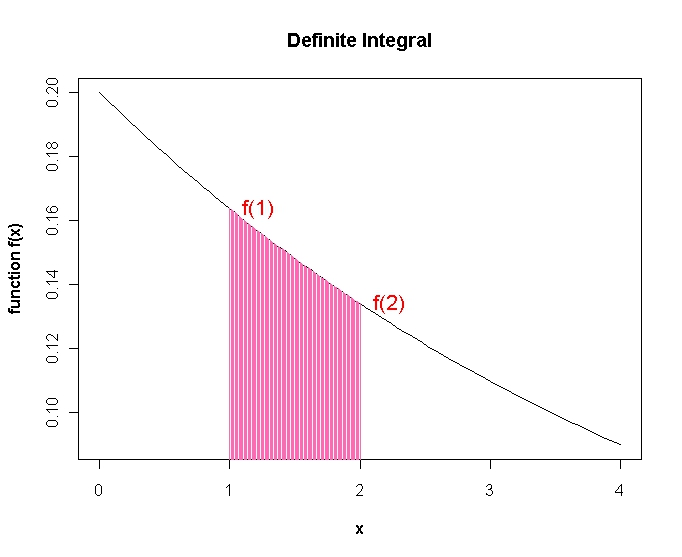
\includegraphics[scale=0.35]{images/6ADefiniteIntegral}
\end{center}
Definite integral of function is area under curve between X=1 and X=2.
%% ----------------------------------%%
%----------------------------------------------------------------------------------------------------%
%% ----------------------------------%%
%% \frametitle{Definite Integral}
\begin{itemize}
	\item Definite integrals are used to compute the ``\textbf{\textit{area under curves}}".
	\item Definite integrals are defined by a lower and upper limit.
	\item The area under the curve between X=1 and  X=2 is depicted in the previous slide.
	\item By computing the definite integral, we are able to determine a value for this area.
	\item Probability can be represented as an area under a curve.
\end{itemize}
%% ----------------------------------%%

%----------------------------------------------------------------------------------------------------%
{\LARGE
	
	%% \frametitle{Probability Density Function}
	\begin{itemize}
		\item
		In probability theory, a \textbf{\emph{probability density function}} (PDF) (or ``density" for short ) of a continuous random variable is a function that describes the relative likelihood for this random variable to occur at a given point.
		
		\item The PDF for a continuous random variable $X$ is often denoted $f(x)$.
		
		\item The probability density function can be integrated to obtain the probability that the random variable takes a value in a given interval.
		
		\item The probability for the random variable to fall within a particular interval is given by the integral of this variable's density over the region.
		
		\item The probability density function is non-negative everywhere, and its integral over the entire space is equal to one.
	\end{itemize}
}

%% ----------------------------------%%

%% \frametitle{Density Curves}


\begin{itemize}
	\item A plot of the PDF is referred to as a `\textbf{\emph{density curve}}'.
	\item A density curve that is always on or above the horizontal axis and has total area underneath equal to one.
	\item Area under the curve in a range of values indicates the proportion of values in that range.
	\item Density curves come in a variety of shapes, but the normal distribution's bell-shaped densities are perhaps the most commonly encountered.
	\item Remember the density is only an approximation, but it simplifies analysis and is generally accurate enough for practical use.
\end{itemize}
%% ----------------------------------%%

%----------------------------------------------------------------------------------------------------%
{\LARGE
	%% \frametitle{The Cumulative Distribution Function }
	Recall:
	\begin{itemize}
		\item The \textbf{\emph{cumulative distribution function}} (CDF), (or just distribution function), describes the probability that a continuous random variable X with a given probability distribution will be found at a value less than or equal to x.\\
		
		\[ F(x) = P(X \leq x) \]
		
		\item Intuitively, it is the ``area so far" function of the probability distribution.
	\end{itemize}
}
%----------------------------------------------------------------------------------------------------%
%% ----------------------------------%%
%% \frametitle{Cumulative Distribution Function}
\vspace{-0.5cm}
\begin{center}
	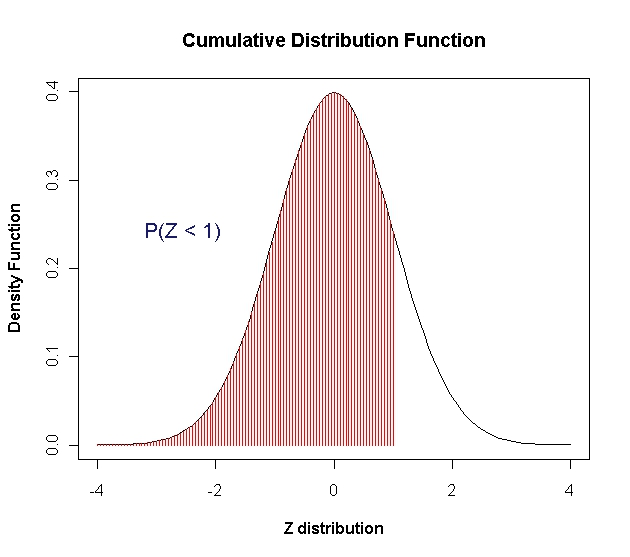
\includegraphics[scale=0.35]{images/6ACDF}
\end{center}
Cumulative Distribution Function $P(Z \leq 1)$ \\ Here the random variable is called $Z$ (we will see why later)
%% ----------------------------------%%



%---------------------------------------------------------------------------%
{\LARGE
	%% \frametitle{Continuous Random Variables}
	
	\begin{itemize}
		\item Probability Density Function
		\item Cumulative Density Function
	\end{itemize}
	
	
	If X is a continuous random variable then we can say that the probability of obtaining a \textbf{precise} value $x$ is infinitely small, i.e. close to zero.
	
	\[P(X=x) \approx 0 \]
	
	Consequently, for continuous random variables (only),  $P(X \leq x)$ and $P(X < x)$ can be used interchangeably.
	
	\[P(X \leq x) \approx P(X < x) \]
	
	
}

%---------------------------------------------------------------------------%
{\LARGE
	%% \frametitle{Continuous Uniform Distribution}
	A random variable X is called a continuous uniform random variable over the interval $(a,b)$ if it's probability density function is given by
	
	\[ f_{X}(x)  =  { 1 \over b-a}   \hspace{2cm}  \mbox{ when } a \leq x \leq b\]
	
	The corresponding cumulative density function is
	
	\[ F_x(x) = { x-a \over b-a}   \hspace{2cm}  \mbox{ when } a \leq x \leq b\]
	
}

%-----------------------------------------------------------------------------%

{\LARGE
	
	The mean of the continuous uniform distribution is
	
	\[ E(X) = {a+b \over 2}\]
	
	\[ V(X) = {(b-a)^2\over12}\]
}

%-----------------------------------------------------------------------------%

{\LARGE
	%% \frametitle{The Memoryless property}
	The most interesting property of the exponential distribution is the \textbf{\emph{memoryless}} property. By this , we mean that if  the lifetime of a component is exponentially distributed, then an item which has been in use for some time is a good as a brand new item with regards to the likelihood of failure.
	
	The exponential distribution is the only distribution that has this property.
}

%--------------------------------------------------------%
\section*{Session 09: Probability}
\begin{itemize}
	\item[9A.1] Counting Methods
	\item[9A.2] Counting using Sets
	\item[9A.3] Probability
	\item[9A.4] Independent Events
\end{itemize}
\begin{itemize}
	\item[9B.1] Permutation
	
	\[ {n \choose r} = \frac{n!}{(n-r)! r!} \]
	
	
	\[ {6 \choose 3} = \frac{6!}{(6-3)! 3!} = \frac{6!}{3! \times 3!}\]
	
	
	\[ \frac{6!}{3! \times 3!} = \frac{6 \times 5 \times 4 \times 3!}{3! \times 3!} = \frac{120}{6} = 120\]
\end{itemize}

%\begin{multicol}{2}
\begin{itemize}
	\item ${6 \choose 2} = 15$
	\item ${5 \choose 2} = 10$  
	\item ${4 \choose 0} = 1$  
	\item ${4 \choose 3} = 4$  
\end{itemize}
%\end{multicol}

\begin{itemize}
	\item pairwise disjoint sets
	\item The addition principle
\end{itemize}
\subsection*{Theorem}
\[ |A \cup B| = |A| + |B| - |A \cap B|  \]

\subsection*{Probability}
\begin{itemize}
	\item[9B.2] The sample space of an experiment ($S$)
	\item[9B.3] The size of a sample space
	\item[9B.4] Indepedent Evcents (9.3.1)
\end{itemize}
%------------------------------------------------%
\section*{Session 9 Probability}
%------------------------------------------------------------%
{ \Large
	%---------------------------% \frametitle{Random Variables}
	\begin{itemize} \item The outcome of an experiment need not be a number, for example, the outcome when a coin is tossed can be `heads' or `tails'. \item
		However, we often want to represent outcomes as numbers. \item
		A \textbf{\emph{random variable}} is a function that associates a unique numerical value with every outcome of an experiment.
		\item The value of the random variable will vary from trial to trial as the experiment is repeated.
		\item Numeric values can be assigned to outcomes that are not usually considered numeric. \item For example, we could assign a `head' a value of $0$, and a `tail' a value of $1$, or vice versa.
	\end{itemize}
}
%------------------------------------------------------------%
{ \Large
	%---------------------------% \frametitle{Random Variables}
	There are two types of random variable - discrete and continuous. The distinction between both types will be important later on in the course.\\ \bigskip
	
	\textbf{Examples}
	\begin{itemize}
		\item A coin is tossed ten times. The random variable X is the number of tails that are noted.
		X can only take the values $\{0, 1, ..., 10\}$, so $X$ is a discrete random variable.
		\item A light bulb is burned until it burns out. The random variable Y is its lifetime in hours.
		Y can take any positive real value, so Y is a continuous random variable.
	\end{itemize}
}

%--------------------------------------------------------------------------------%
{ \Large
	%---------------------------% \frametitle{Discrete Random Variable}
	\begin{itemize}
		\item A discrete random variable is one which may take on only a countable number of distinct values such as $\{0, 1, 2, 3, 4, ... \}$.\item Discrete random variables are usually (but not necessarily) counts. \item If a random variable can take only a finite number of distinct values, then it must be discrete. \item Examples of discrete random variables include the number of children in a family, the Friday night attendance at a cinema, the number of patients in a doctor's surgery, the number of defective light bulbs in a box of ten.
	\end{itemize}
}


%--------------------------------------------------------------------------------%
{ \Large
	%---------------------------% \frametitle{Continuous Random Variable}
	\begin{itemize} \item
		A continuous random variable is one which takes an infinite number of possible values. \item Continuous random variables are usually measurements. \item Examples include height, weight, the amount of sugar in an orange, the time required to run a computer simulation. \end{itemize}
	
}
	
	%=================================================================== %
	%--------------------------------------%
	
	%---------------------------% \frametitle{Random Variables}
	A pair of dice is thrown. Let X denote the minimum of the two numbers which occur.
	Find the distributions and expected value of X.
		A fair coin is tossed four times.
	Let X denote the longest string of heads.
	Find the distribution and expectation of X.

A fair coin is tossed until a head or five tails occurs.
	Find the expected number E of tosses of the coin.
	%--------------------------------------%
	%=================================================================== %
	%--------------------------------------%
	%---------------------------% \frametitle{Random Variables}A coin is weighted so that P(H) = 0.75 and P(T ) = 0.25
	
	The coin is tossed three times. Let X denote the number of
	heads that appear.
	\begin{itemize}
		\item (a) Find the distribution f of X.
		\item (b) Find the expectation E(X).
	\end{itemize}
	
	%--------------------------------------%
	%=================================================================== %
	%--------------------------------------%
	%---------------------------% \frametitle{Graphical Procedures for Statistics}
	\begin{itemize}
		\item Bar-plots
		\item Histograms
		\item Boxplots
		
	\end{itemize}
	
	%--------------------------------------%
	%=================================================================== %
	%--------------------------------------%
	%---------------------------% \frametitle{Histograms}
	\begin{itemize}
		\item Consider an experiment in which each student in a class of 60 rolls a die 100 times.
		\item Each score is recorded, and a total score is calculated.
		\item As the expected value of rolled die is 3.5, the expected total is 350 for each student.
		\item At the end of the experiment the students reported their totals.
		\item The totals were put into ascending order, and tabulated as follows (next slide).
	\end{itemize}
	
	
	%--------------------------------------%
	%=================================================================== %
	%--------------------------------------%
	%---------------------------% \frametitle{Outcomes of die-throw experiment}
	\small
	\begin{center}
		\begin{tabular}{|c c c c c c c c c c|}
			\hline
			% after \\: \hline or \cline{col1-col2} \cline{col3-col4} ...
			307 & 321 & 324 & 328 & 329 & 330 & 334 & 335 & 336 &337 \\
			337 & 337 & 338 & 339 & 339 & 342 & 343 & 343 & 344 &344 \\
			346 & 346 & 347 & 348 & 348 & 348 & 350 & 351 & 352 &352 \\
			353 & 353 & 353 & 354 & 354 & 356 & 356 & 357 & 357 &358 \\
			358 & 360 & 360 & 361 & 362 & 363 & 365 & 365 & 369 &369 \\
			370 & 370 & 374 & 378 & 381 & 384 & 385 & 386 & 392 &398 \\
			\hline
		\end{tabular}
	\end{center}
	\normalsize
	\begin{itemize}
		\item What proportion of outcomes are less than or equal to 330? \\ (Answer: $10\%$)
		\item What proportion of outcomes are greater than or equal to 370?\\ (Answer: $16.66\%$)
	\end{itemize}
	
	%--------------------------------------%
	%=================================================================== %
	%--------------------------------------%
	%---------------------------% \frametitle{What is a Histograms}
	
	TEXT HERE
	
	
	%--------------------------------------%
	%=================================================================== %
	%--------------------------------------%
	%---------------------------% \frametitle{Histograms}
	For the die-throw experiment;
	\begin{center}
		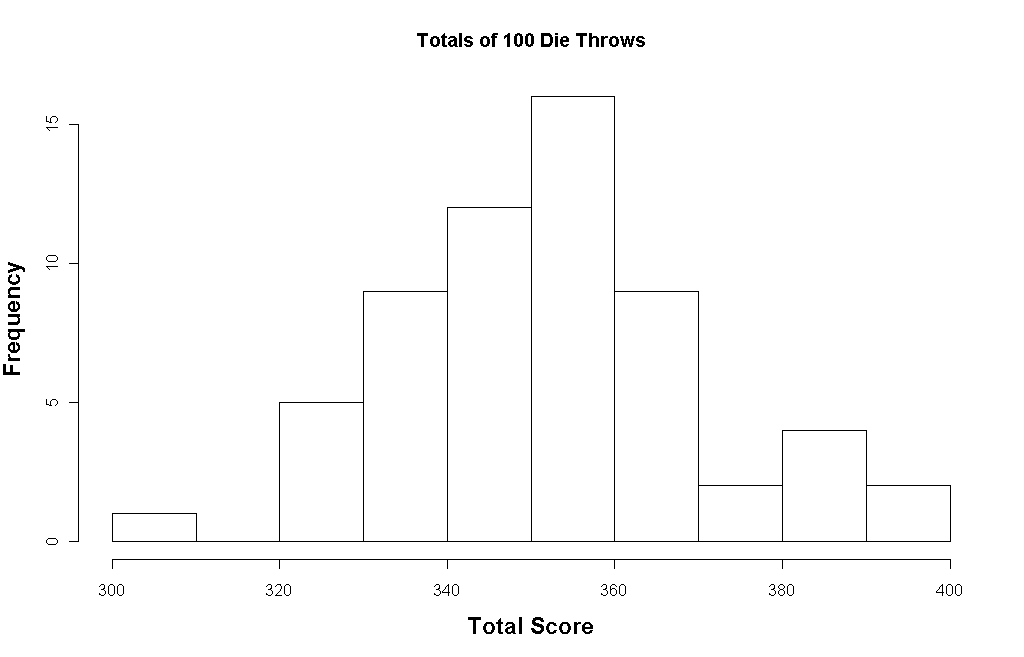
\includegraphics[scale=0.30]{images/3aDieHist}
	\end{center}
	
	
	%--------------------------------------%
	%=================================================================== %
	%--------------------------------------%
	%---------------------------% \frametitle{Constructing Histograms}
	\begin{itemize}
		\item Compute an appropriate number of class intervals.
		\item As a rule of thumb, the number of class intervals is usually approximately the square root of the number of observations.
		\item As there are 60 observations, we would normally use 7 or 8 class intervals.
		\item To save time, we will just use 5 class intervals.
	\end{itemize}
	
	%--------------------------------------%
	
	%=================================================================== %
	%--------------------------------------%
	
	%---------------------------% \frametitle{Histograms}
	
	\begin{center}
		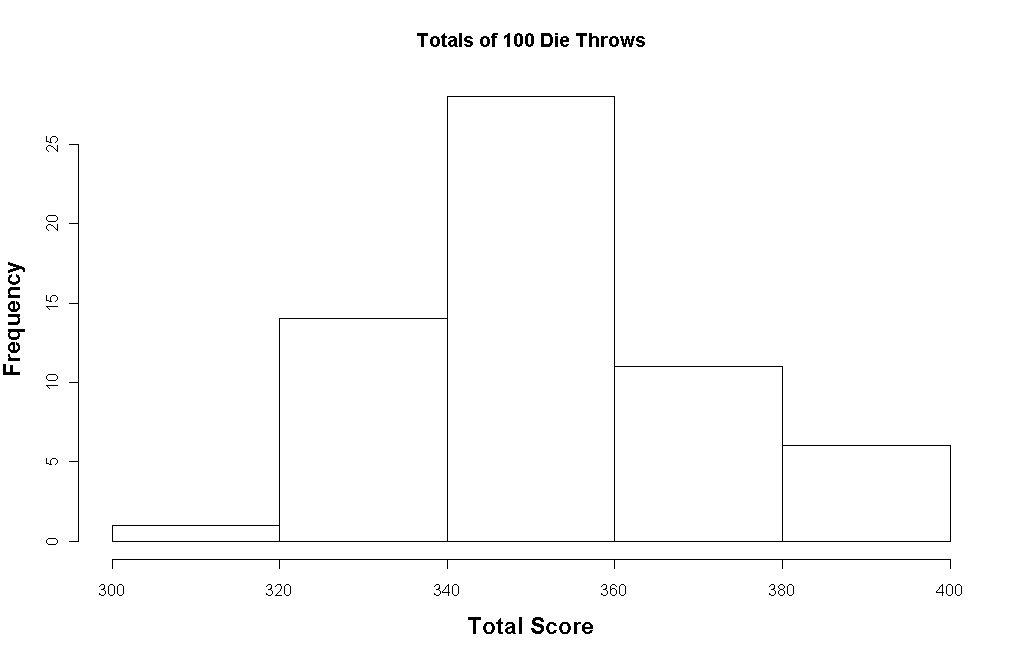
\includegraphics[scale=0.30]{images/3aDieHist2}
	\end{center}
	
	
	%--------------------------------------%
	%=================================================================== %
	%--------------------------------------%
	%---------------------------% \frametitle{Histograms}
	\begin{itemize}
		\item Suppose that the experiment of throwing a die 100 times and recording the total was repeated 100,000 times.
		\item (If implemented on a computer, we would call this a simulation study)
		\item The histogram of data (with a class interval width of 2) is shown on the next slide.
		\item How should the shape of the histogram be described?
		\item ``Bell-shaped" would be a suitable description.
	\end{itemize}
	
	%--------------------------------------%
	%=================================================================== %
	%--------------------------------------%
	%---------------------------% \frametitle{Histograms}
	
	\begin{center}
		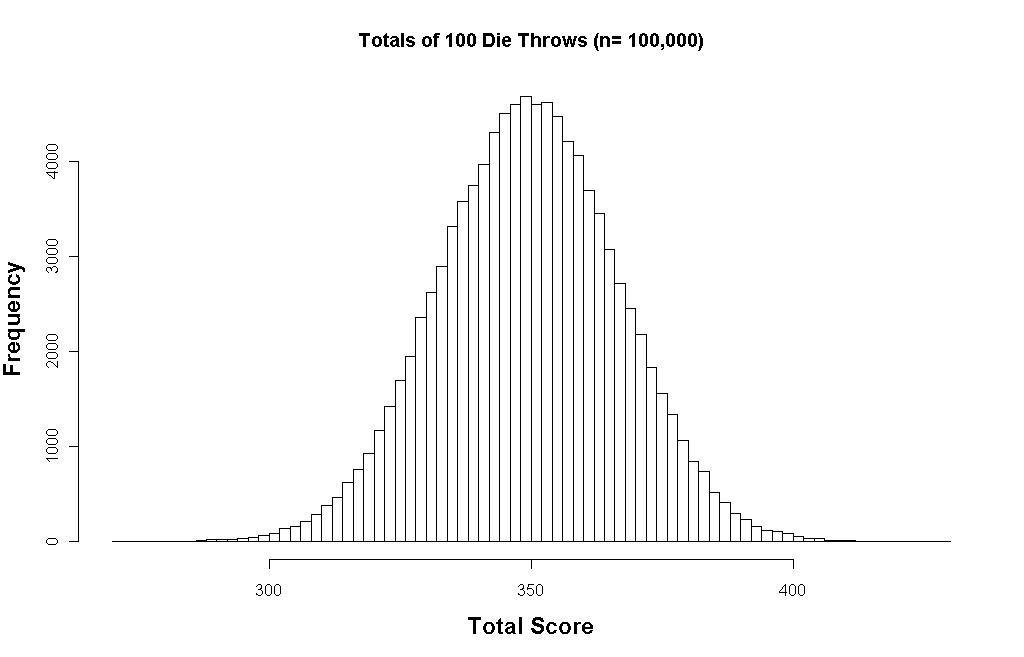
\includegraphics[scale=0.30]{images/3aDieHist3}
	\end{center}
	
	
	%--------------------------------------%
	%=================================================================== %
	%--------------------------------------%
	%---------------------------% \frametitle{Simulation Study}
	A couple of remarks about the simulation study, some of which will be relevant later on.
	\begin{itemize}
		% \item Approximately 76\% of the values are between 330 and 370.
		\item Approximately 68.7\% of the values in the simulation study are between 332 and 367.
		\item Approximately 95\% of the values are between 316 and 383.
		\item $2.5\%$ of the values output are less than 316.
		\item $2.5\%$ of the values study output are greater than 383.
		\item 175 values are greater than or equal to 400, whereas 198 values are less than or equal to 300.
		\item Results such as these are unusual, but they are not impossible.
	\end{itemize}
	
	%--------------------------------------%
	%=================================================================== %
	%--------------------------------------%
	%---------------------------% \frametitle{Random Variables}
	A pair of dice is thrown. Let X denote the minimum of the two numbers which occur.
	Find the distributions and expected value of X.
	
	%--------------------------------------%
	%=================================================================== %
	%--------------------------------------%
	%---------------------------% \frametitle{Random Variables}
	A fair coin is tossed four times.
	Let X denote the longest string of heads.
	Find the distribution and expectation of X.
	
	%--------------------------------------%
	%=================================================================== %
	%--------------------------------------%
	%---------------------------% \frametitle{Random Variables}
	A fair coin is tossed until a head or five tails occurs.
	Find the expected number E of tosses of the coin.
	%--------------------------------------%
	%=================================================================== %
	%--------------------------------------%
	%---------------------------% \frametitle{Random Variables}A coin is weighted so that P(H) = 0.75 and P(T ) = 0.25
	
	The coin is tossed three times. Let X denote the number of
	heads that appear.
	\begin{itemize}
		\item (a) Find the distribution f of X.
		\item (b) Find the expectation E(X).
	\end{itemize}
	
	%--------------------------------------%
	%=================================================================== %
	%--------------------------------------%
	\begin{itemize}
		\item Now consider an experiment with only two outcomes. Independent repeated trials of such an experiment are
		called Bernoulli trials, named after the Swiss mathematician Jacob Bernoulli (1654–1705). \item The term \textbf{\emph{independent
				trials}} means that the outcome of any trial does not depend on the previous outcomes (such as tossing a coin).
		\item We will call one of the outcomes the ``success" and the other outcome the ``failure".
	\end{itemize}
	
	%--------------------------------------%
	%=================================================================== %
	%--------------------------------------%
	\begin{itemize} \item
		Let $p$ denote the probability of success in a Bernoulli trial, and so $q = 1 - p$ is the probability of failure.
		A binomial experiment consists of a fixed number of Bernoulli trials. \item A binomial experiment with $n$ trials and
		probability $p$ of success will be denoted by
		\[B(n, p)\]
	\end{itemize}
	%--------------------------------------%
	%=================================================================== %
	
	\subsection*{Binomial Coefficients}
\begin{itemize}
	\item factorials 
	\[ n! = (n)\times (n-1)\times(n-2) \times \ldots \times 1 \]
	\begin{itemize}
		\item $5! = 5 \times 4 \times 3 \times 2 \times 1 = 120 $
		\item $3! = 3 \times 2 \times 1$
	\end{itemize}
	\item Zero factorial
	\[ 0! =  1 \]
\end{itemize}
%---------------------------------------------- %

% \[P(A |B = \frac{P(A \cap B)}{P(B)})\]

The complement rule in Probability

$P(C^{\prime}) = 1- P(C)$


%--------------------------------------------------------------------------------------%
{ \Large
	%%- \frametitle{Discrete Probability Distributions}
	
	\begin{itemize}
		
		\item Over the next set of lectures, we are now going to look at two important discrete probability distributions
		
		\item The first is the \textbf{\emph{binomial}} probability distribution.
		
		\item The second is the Poisson probability distribution.
		
		\item In \texttt{R}, calculations are performed using the \texttt{binom} family of functions and \texttt{pois} family of functions respectively.
		
		\item Now consider an experiment with only two outcomes. Independent repeated trials of such an experiment are
		called Bernoulli trials, named after the Swiss mathematician Jacob Bernoulli (1654–1705). \item The term \textbf{\emph{independent
				trials}} means that the outcome of any trial does not depend on the previous outcomes (such as tossing a coin).
		\item We will call one of the outcomes the ``success" and the other outcome the ``failure".
		
		\item
		Let $p$ denote the probability of success in a Bernoulli trial, and so $q = 1 - p$ is the probability of failure.
		A binomial experiment consists of a fixed number of Bernoulli trials. \item A binomial experiment with $n$ trials and
		probability $p$ of success will be denoted by
		\[B(n, p)\]
		\item a probability mass function (pmf) is a function that gives the probability that a 
		discrete random variable is exactly equal to some value. 
		\item The probability mass function is often the primary means of defining a discrete probability distribution 
	\end{itemize}
}
%------------------------------------------------------------------%
{ \Large
	Thirty-eight students took the test. The X-axis shows various intervals of scores (the interval labeled 35 includes any score from 32.5 to 37.5). The Y-axis shows the number of students scoring in the interval or below the interval.
	
	\textbf{\emph{cumulative frequency distribution}}A  can show either the actual frequencies at or below each interval (as shown here) or the percentage of the scores at or below each interval. The plot can be a histogram as shown here or a polygon.
}




		\section*{Session 09: Probability}
		\begin{itemize}
			\item[9B.1] Permutation
			
			\[ {n \choose r} = \frac{n!}{(n-r)! r!} \]
			
			
			\[ {6 \choose 3} = \frac{6!}{(6-3)! 3!} = \frac{6!}{3! \times 3!}\]
			
			
			\[ \frac{6!}{3! \times 3!} = \frac{6 \times 5 \times 4 \times 3!}{3! \times 3!} = \frac{120}{6} = 120\]
		\end{itemize}
		
		%\begin{multicol}{2}
		\begin{itemize}
			\item ${6 \choose 2} = 15$
			\item ${5 \choose 2} = 10$  
			\item ${4 \choose 0} = 1$  
			\item ${4 \choose 3} = 4$  
		\end{itemize}
		%\end{multicol}
		
		\begin{itemize}
			\item pairwise disjoint sets
			\item The addition principle
		\end{itemize}
		\subsection*{Theorem}
		\[ |A \cup B| = |A| + |B| - |A \cap B|  \]
		
		\subsection*{Probability}
		\begin{itemize}
			\item[9B.2] The sample space of an experiment ($S$)
			\item[9B.3] The size of a sample space
			\item[9B.4] Indepedent Evcents (9.3.1)
		\end{itemize}
		%------------------------------------------------%
		
		
		%---------------------------------------------------- %
		%SLIDE1 - GOOD
		\Large
		Suppose an electronics assembly subcontractor receives resistors from two suppliers: A and B
		
		\begin{itemize}
			\item Supplier A supplies 80\% of the resistors
			\vspace{2cm}
			\item Supplier B supplies 20\% of the resistors
			\vspace{2cm}
		\end{itemize}
		
		
		%SLIDE2 - Slide 1 with reveal - GOOD
		\Large
		Suppose an electronics assembly subcontractor recieves resistors from two suppliers A and B
		
		\begin{itemize}
			\item Supplier A supplies 80\% of the resistors
			{
				\Large
				
				\item \textit{Probability that a randomly chosen resistor comes from A is 80 \%}
				\item \textit{P(A) = 0.80 }
				
			}
			\item Supplier B supplies 20\% of the resistors
			\item \textit{Probability that a randomly chosen resistor comes from B is therefore 20\%}
			\item \textit{P(B) = 0.20}
		\end{itemize}
		
		%----------------------------------------------------- %
		% Slide 4
		\Large
		\begin{itemize}
			\item We are giving information about the rate of faulty components from each supplier. \\(Faulty : resistor fails some quality test)
			\vspace{1cm}
			\item 1\% of the resistors supplied by A are faulty
			\vspace{1cm}
			\item 3\% of the resistors supplied by B are faulty 
			\vspace{1cm}
		\end{itemize}
		
		%-----------------------------------------------------%
		% Slide 4 - Slide 3 with Reveal
		\Large
		\begin{itemize}
			\item We are giving information about the rate of faulty components from each supplier. \\(Faulty : resistor fails some quality test)
			\item  \textit{P(F) probability that randomly selecting compoent is faulty}
			\item 1\% of the resistors supplied by A are faulty.
			\item\textit{ We write this as $P(F|A) =0.01$}
			\item 3\% of the resistors supplied by B are faulty 
			\item \textit{We write this as $P(F|B) =0.03$}
		\end{itemize}
		
		%-----------------------------------------------------%
		% Slide 5 Good
		\Large
		\vspace{-1.5cm}
		\textbf{Question 1:}
		\begin{itemize}
			\item What is the probability that a randomly selected resistor fails the final test?
			
			\item In mathematical terms, compute P(F) 
		\end{itemize}
		
		
		
		%------------------------------------------------------%
		
		
		\Large
		\textbf{Law of Total Probability:}
		\begin{itemize}
			\item Faulty Resistors are either from Supplier A or Supplier B.
			\vspace{0.3cm} 
			\item \textit{Resistors MUST come from one of the two suppliers.}
			\item \textit{A and B are mutually exclusive.}
		\end{itemize}
		\vspace{0.3cm} 
		\[ P(F) = P(F \mbox{ and } A) + P(F \mbox{ and } B) \]
		
		
		
		
		\Large
		\textbf{Conditional Probability}
		
		\[ P(X|Y)  = \frac{P(X \mbox{ and } Y)}{P(Y)} \]
		
		Re-arranging
		\[ P(X \mbox{ and } Y) =  P(X|Y)\times P(Y) \]
		Therefore we can say
		\[ P(F \mbox{ and } A) =  P(F|A)\times P(A) \]\\
		\[ P(F \mbox{ and } B) =  P(F|B)\times P(B) \]
		
		
		
		\Large
		\vspace{-1.5cm}
		\[ P(F \mbox{ and } A) =  P(F|A)\times P(A) \]\\
		\vspace{1.7cm}
		\[ P(F \mbox{ and } B) =  P(F|B)\times P(B) \]
		
		
		
		\Large
		\[ P(F \mbox{ and } A) =  P(F|A)\times P(A) = 0.80 \times 0.01\]\\
		\[ P(F \mbox{ and } A) = 0.008\]
		\bigskip
		\[ P(F \mbox{ and } B) =  P(F|B)\times P(B) = 0.20 \times 0.03\]\\
		\[ P(F \mbox{ and } B) = 0.006\]
		
%=================================================================================================$		
		\textbf{Recall:}
		\[ P(F) = P(F \mbox{ and } A) + P(F \mbox{ and } B) \]
		
		
		
		\newpage
		\section*{Session 9 Probability}

		%---------------------------------------------- %
		
		% \[P(A |B = \frac{P(A \cap B)}{P(B)})\]
		
		The complement rule in Probability
		
		$P(C^{\prime}) = 1- P(C)$
		
		
		
		If the probability of C is $70 \%$ then the probability of $C^{\prime}$ is $30\%$
		
		
		%-----------------------------------------%
		\newpage
%-----------------------------------------------------%


\large
\begin{itemize}
	\item Permutations where repetition is allowed: 
	\[ n! \]
	\item Permutations where repetition is not allowed
	\[ \frac{n!}{(n-k)!} \]
	\end{itemize}
	
	
	%-----------------------------------------------------%
	
	% http://www.hss.caltech.edu/~mshum/stats/lect2.pdf
	
	
	
	\bigskip
	{
		\huge
		\[ \mbox{Expected Values of Random Variables}\]
		\Large
		\[ \mbox{Example Exercise}\]
		\bigskip
		\Large
		\[ \mbox{www.MathsResource.com}\]
	}
	
	
	
	%\frametitle{Expected Values of Random Variables}
	\Large
	If the random variable $Z$ has a distribution which is standard normal, show that the expected value of $e^{sZ}$ is given as follows:
	
	{
		\LARGE
		\[E(e^{sZ})  =  e^{\frac{s^2}{2}}\] 
	}
	
	
	
	%---------------------------------------------------- %
	
	
	%\frametitle{Expected Values of Random Variables}
	\Large
	\begin{itemize}
		\item In general, the expected value is computed using this formula
		{
			\LARGE
			\[ E(X) =  \int_{-\infty}^{\infty}  x \times f(x) dx   \]
		}
		\item The expected value of a \textbf{\textit{transformed}} random variable is computed using this formula
		{
			\LARGE
			\[ E( tf(X) ) =  \int_{-\infty}^{\infty}  tf(x) \times f(x) dx   \]
		}
	\end{itemize}
	
	
	%---------------------------------------------------- %
	
	
	%\frametitle{Expected Values of Random Variables}
	\Large
	\begin{itemize}
		\item 
		The probability density function for the standard normal distribution is
		{
			\Large
			\[f(x, \mu, \sigma) = \frac{1}{\sigma\sqrt{2\pi}} e^{ -\frac{(x-\mu)^2}{2\sigma^2} }\]}
		\item 
		The probability density function for the standard normal distribution is
		{
			\Large
			\[f(z) = f(x, \mu= 0, \sigma=1) = \frac{1}{\sqrt{2\pi}} e^{ -{x \over 2}^2 }\]
		}
	\end{itemize}
	
	%---------------------------------------------------- %
	
	%\frametitle{Expected Values of Random Variables}
	\Large
	%\vspace{-4cm}
	
	
	
	{
		\LARGE
		\[ E( e^{sZ} ) =  \int_{-\infty}^{\infty}  e^{sx} \;\times\; \frac{1}{\sqrt{2\pi}} \;e^{ -{x \over 2}^2 }\]
	}
	
	
	
	%---------------------------------------------------- %
	
	%\frametitle{Expected Values of Random Variables}
	\Large
	%\vspace{-4cm}
	
	
	
	{
		\LARGE
		\[ E( e^{sZ} ) =  \frac{1}{\sqrt{2\pi}} \int_{-\infty}^{\infty}   e^{ \big[sx-\frac{(x)^2}{2} \big]} dx   \]
	}
	
	
	%---------------------------------------------------- %
	
	%\frametitle{Expected Values of Random Variables}
	\Large
	%\vspace{-4cm}
	
	
	
	{
		\LARGE
		\[ E( e^{sZ} ) =  e^{{s^2\over 2}} \; \times\; \frac{1}{\sqrt{2\pi}} \int_{-\infty}^{\infty} e^{ \big[-\frac{(x-s)^2}{2} \big]} dx   \]
	}
	
	
	%---------------------------------------------------- %
	
	%\frametitle{Expected Values of Random Variables}
	\Large
	%\vspace{-3cm}
	\textbf{Mathematical Identity}
	\begin{itemize}
		\item Proven in a separate video
	\end{itemize}
	{
		\LARGE
		\[\int_{-\infty}^{\infty} e^{-{y\over 2}^2}dy  = \sqrt{2\pi}\]
		
	}
	
	
	%---------------------------------------------------- %
	
	%\frametitle{Expected Values of Random Variables}
	\Large
	%\vspace{-2.5cm}
	
	
	
	{
		\LARGE
		\[ E( e^{sZ} ) =  e^{{s^2\over 2}} \; \times\; \frac{1}{\sqrt{2\pi}} \int_{-\infty}^{\infty} e^{ \big[-\frac{(x-s)^2}{2} \big]} dx \]
		
		
		\[ E( e^{sZ} ) =  e^{{s^2\over 2}} \; \times\; \frac{1}{\sqrt{2\pi}} \big[\sqrt{2\pi} \big] \]
	}
	
	
	
	
	Suppose an electronics assembly subcontractor recieves resistors from two suppliers A and B
	
	Supplier A supplies 80% of the resistors
	
	P(A) = 0.80 probability that a randomly chosen resistor comes from A
	
	Supplier B supplies 20% of the resistors
	
	P(B) = 0.20 probability that a randomly chosen resistor comes from B
	
	
	%-----------------------------------------------------%
	
	\Large
	\begin{itemize}
		\item 1% of the resistors supplied by A are faulty (i.e. resistor fails the final test)
		\item 3% of the resistors supplied by B are faulty 
	\end{itemize}
	
	%-----------------------------------------------------%
	
	
	Qeustion: What is the probability that a randomly selected resistor fails the final test?
	
	Compute P(F) 
	
	
	%------------------------------------------------------%
	
	
	\Large
	P(F) = P(FandA) + P(FandB)
	
	
	





%\frametitle{Probability Distribution}

%--------------------------------------%





%---------------------------------------%

A probability distribution is a mathematical approach to quantifying uncertainty.

There are two main classes of probability distributions: Discrete and continuous. 

Discrete distributions describe variables that take on discrete values only (typically the positive integers), while continuous 
distributions describe variables that can take on arbitrary values in a continuum (typically the real numbers).








%---------------------------------------%






Binomial Distribution

A manufacturer of hospital equipment knows from experience that 5% of the production will have some type of minor default, and will require adjustment.

Number of independent trials    n

Probability of a "success" p






%\frametitle{Poisson Distribution}

%--------------------------------------%





%---------------------------------------%

A basic introduction to the concept

Example

Certain events happen at unpredictable intervals. But for some reason, no matter how recent or long ago last event was, the probability that another event will occur within the next hour is exactly the same (say, 10%). The same holds for any other time interval (say, second). Moreover, the number of events within any given time interval is statistically independent of numbers of events in other intervals that do not overlap the given interval. Also, two events never occur simultaneously.

Then the number of events per day is Poisson distributed.

%---------------------------------------%
Formal definition

Let X be a stochastic variable taking non-negative integer values with probability density function

\[ P(X=k)=f(k)= e^{-\lambda} \frac{\lambda ^k}{k!}.\] 
Then X follows the Poisson distribution with parameter $\lambda$.

%---------------------------------------%
Characteristics of the Poisson distribution

If X is a Poisson distribution stochastic variable with parameter $\lambda$, then

\begin{itemize}
	\item The expected value $E[X]=\lambda$
	\item The variance $Var[X]=\lambda$
\end{itemize}
%----------------------------------------%





\huge
\[ \mbox{The Normal Distribution} \]
\Large
\[ \mbox{Symmetric Intervals} \]




%---------------------------------------------------%



Symmetric Intervals

\[ P( -z \leq Z \leq z) \]



%---------------------------------------------------%




%---------------------------------------------------%



\huge
\[ \mbox{The Normal Distribution} \]
\Large
\[ \mbox{The Symmetry Rule} \]




%---------------------------------------------------%



\huge
\[ \mbox{The Normal Distribution} \]
\Large
\[ \mbox{The Symmetry Rule} \]


%---------------------------------------------------%

%\frametitle{Normal Distribution : The Symmetry Rule}
\Large
From statistical tables, we could determine the following:
\begin{itemize}
	\item $P(Z \leq 1.5) $
	\item $P(Z \geq 1.5) $
\end{itemize}


%---------------------------------------------------%

%\frametitle{Normal Distribution : The Symmetry Rule}
\Large

Consider the normally distributed random variable $X$

\[ X \sim \mathcal{N}(\mu=1000,\sigma^2 = 2500) \]

Paramters:
\begin{itemize}
	\item $\mu =1000$
	\item $\sigma =50$
\end{itemize}
Questions

\begin{itemize}
	\item $P(X \leq 925)$
	\item $P(X \geq 925)$
\end{itemize}



%---------------------------------------------------%

%\frametitle{Normal Distribution : The Symmetry Rule}
\textbf{Z-score}
\[ z =\frac{x - \mu}{\sigma}\]

\[ X \sim \mathcal{N}(\mu=1000,\sigma^2 = 2500) \]

\begin{itemize}
	\item Mean $\mu= 1000$
	\item Standard Deviation $\sigma = 50$
\end{itemize}

%---------------------------------------------------%

%\frametitle{Normal Distribution : The Symmetry Rule}

\[ P(X \leq 925)  = P(Z \leq -1.5) \]

Applying the Symmetry Rule
\[ P(Z \leq -1.5) = P(Z \geq 1.5) = 0.0668\]

Theerefore we can say 
\[ P(X \leq 925) = 0.0668 \]

%---------------------------------------------------%

%\frametitle{Standardizing normal random variables}

As a consequence of Property 1, it is possible to relate all normal random variables to the standard normal.

If $X \sim N(\mu, \sigma^2)$, then

\[Z = \frac{X - \mu}{\sigma} \]
is a standard normal random variable: $Z \sim N(0,1)$. An important consequence is that the cdf of a general normal distribution is therefore

\[\Pr(X \le x)
=
\Phi
\left(
\frac{x-\mu}{\sigma}
\right)
=
\frac{1}{2}
\left(
1 + \operatorname{erf}
\left(
\frac{x-\mu}{\sigma\sqrt{2}}
\right)
\right)\]
.


%-------------------------------------------------------------------------%


Conversely, if Z is a standard normal distribution, $Z \sim N(0,1)$, then

\[X = \sigma Z + \mu\]
is a normal random variable with mean $\mu$ and variance $\sigma^2$.

The standard normal distribution has been tabulated (usually in the form of value of the cumulative distribution function F), and the other normal distributions are the simple transformations, as described above, of the standard one. Therefore, one can use tabulated values of the cdf of the standard normal distribution to 
find values of the cdf of a general normal distribution.


%------------------------------------------------------------------------------------------------%
%------------------------------------------------------------------------------------------------%
%------------------------------------------------------------------------------------------------%

\subsection{Statistics}

\begin{enumerate}
	\item Sample mean
	\begin{equation*}
	\bar{x}=\frac{\sum x_{i}}{n}.
	\end{equation*}
	
	\item Sample standard deviation
	\begin{equation*}
	s=\sqrt{\frac{\sum \left( x_{i}-\bar{x}\right) ^{2}}{%
			n-1}}.
	\end{equation*}
	
	\item Conditional probability:
	\begin{equation*}
	P(B|A)=\frac{P\left( A\text{ and }B\right) }{P\left( A\right) }.
	\end{equation*}
	
	
	
	
	
	
\end{enumerate}
		\section*{Complement Rule}
		
		%---------------------------------------------- %
		
		% \[P(A |B = \frac{P(A \cap B)}{P(B)})\]
		
		The complement rule in Probability
		
		$P(C^{\prime}) = 1- P(C)$
		
		
		
		If the probability of C is $70 \%$ then the probability of $C^{\prime}$ is $30\%$

%------------------------------------------------------------%
{\LARGE
	%\frametitle{Random Variables}
	\begin{itemize} \item The outcome of an experiment need not be a number, for example, the outcome when a coin is tossed can be `heads' or `tails'. \item
		However, we often want to represent outcomes as numbers. \item
		A \textbf{\emph{random variable}} is a function that associates a unique numerical value with every outcome of an experiment.
		\item The value of the random variable will vary from trial to trial as the experiment is repeated.
		\item Numeric values can be assigned to outcomes that are not usually considered numeric. \item For example, we could assign a `head' a value of $0$, and a `tail' a value of $1$, or vice versa.
	\end{itemize}
}
%------------------------------------------------------------%
{\LARGE
	%\frametitle{Random Variables}
	There are two types of random variable - discrete and continuous. The distinction between both types will be important later on in the course.\\ \bigskip
	
	\textbf{Examples}
	\begin{itemize}
		\item A coin is tossed ten times. The random variable X is the number of tails that are noted.
		X can only take the values $\{0, 1, ..., 10\}$, so $X$ is a discrete random variable.
		\item A light bulb is burned until it burns out. The random variable Y is its lifetime in hours.
		Y can take any positive real value, so Y is a continuous random variable.
	\end{itemize}
}

%--------------------------------------------------------------------------------%
{\LARGE
	%\frametitle{Discrete Random Variable}
	\begin{itemize}
		\item A discrete random variable is one which may take on only a countable number of distinct values such as $\{0, 1, 2, 3, 4, ... \}$.\item Discrete random variables are usually (but not necessarily) counts. \item If a random variable can take only a finite number of distinct values, then it must be discrete. \item Examples of discrete random variables include the number of children in a family, the Friday night attendance at a cinema, the number of patients in a doctor's surgery, the number of defective light bulbs in a box of ten.
	\end{itemize}
}


%--------------------------------------------------------------------------------%
{\LARGE
	%\frametitle{Continuous Random Variable}
	\begin{itemize} \item
		A continuous random variable is one which takes an infinite number of possible values. \item Continuous random variables are usually measurements. \item Examples include height, weight, the amount of sugar in an orange, the time required to run a computer simulation. \end{itemize}
	
}

		%=================================================================== %
		
		
		%\frametitle{Random Variables}
		A pair of dice is thrown. Let X denote the minimum of the two numbers which occur.
		Find the distributions and expected value of X.
		
		
		%=================================================================== %
		
		%\frametitle{Random Variables}
		A fair coin is tossed four times.
		Let X denote the longest string of heads.
		Find the distribution and expectation of X.
		
		%=================================================================== %
		
		%\frametitle{Random Variables}
		A fair coin is tossed until a head or five tails occurs.
		Find the expected number E of tosses of the coin.
		
		%=================================================================== %
		
		%\frametitle{Random Variables}A coin is weighted so that P(H) = 0.75 and P(T ) = 0.25
		
		The coin is tossed three times. Let X denote the number of
		heads that appear.
		\begin{itemize}
			\item (a) Find the distribution f of X.
			\item (b) Find the expectation E(X).
		\end{itemize}
		
		
		%=================================================================== %
		
		%\frametitle{Graphical Procedures for Statistics}
		\begin{itemize}
			\item Bar-plots
			\item Histograms
			\item Boxplots
			
		\end{itemize}
		
		\begin{itemize}
			\item Consider an experiment in which each student in a class of 60 rolls a die 100 times.
			\item Each score is recorded, and a total score is calculated.
			\item As the expected value of rolled die is 3.5, the expected total is 350 for each student.
			\item At the end of the experiment the students reported their totals.
			\item The totals were put into ascending order, and tabulated as follows (next slide).
		\end{itemize}
		
		
		
		%=================================================================== %
		
		%\frametitle{Outcomes of die-throw experiment}
		\small
		\begin{center}
			\begin{tabular}{|c c c c c c c c c c|}
				\hline
				% after \\: \hline or \cline{col1-col2} \cline{col3-col4} ...
				307 & 321 & 324 & 328 & 329 & 330 & 334 & 335 & 336 &337 \\
				337 & 337 & 338 & 339 & 339 & 342 & 343 & 343 & 344 &344 \\
				346 & 346 & 347 & 348 & 348 & 348 & 350 & 351 & 352 &352 \\
				353 & 353 & 353 & 354 & 354 & 356 & 356 & 357 & 357 &358 \\
				358 & 360 & 360 & 361 & 362 & 363 & 365 & 365 & 369 &369 \\
				370 & 370 & 374 & 378 & 381 & 384 & 385 & 386 & 392 &398 \\
				\hline
			\end{tabular}
		\end{center}
		\normalsize
		\begin{itemize}
			\item What proportion of outcomes are less than or equal to 330? \\ (Answer: $10\%$)
			\item What proportion of outcomes are greater than or equal to 370?\\ (Answer: $16.66\%$)
		\end{itemize}
		
		

		
		
		
		%=================================================================== %
		
		%\frametitle{Constructing Histograms}
		\begin{itemize}
			\item Compute an appropriate number of class intervals.
			\item As a rule of thumb, the number of class intervals is usually approximately the square root of the number of observations.
			\item As there are 60 observations, we would normally use 7 or 8 class intervals.
			\item To save time, we will just use 5 class intervals.
		\end{itemize}
		
		
		
		%=================================================================== %
		
		
		%\frametitle{Histograms}
		
		\begin{center}
			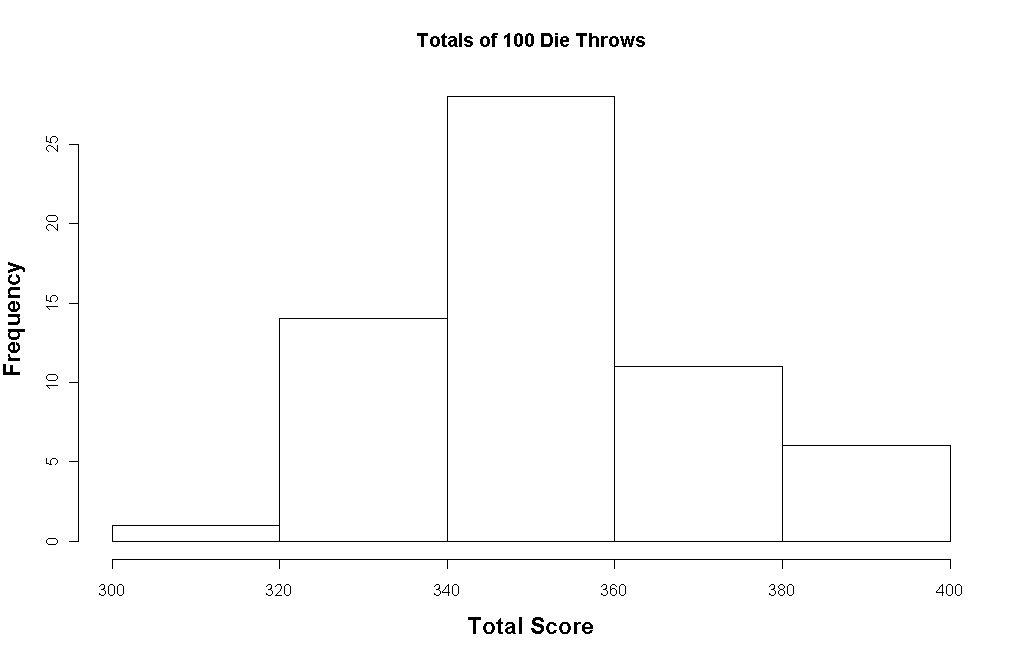
\includegraphics[scale=0.30]{images/3aDieHist2}
		\end{center}
		
		
		
		%=================================================================== %
		
		%\frametitle{Histograms}
		\begin{itemize}
			\item Suppose that the experiment of throwing a die 100 times and recording the total was repeated 100,000 times.
			\item (If implemented on a computer, we would call this a simulation study)
			\item The histogram of data (with a class interval width of 2) is shown on the next slide.
			\item How should the shape of the histogram be described?
			\item ``Bell-shaped" would be a suitable description.
		\end{itemize}
		
		
		%=================================================================== %
		
		%\frametitle{Histograms}
		
		\begin{center}
			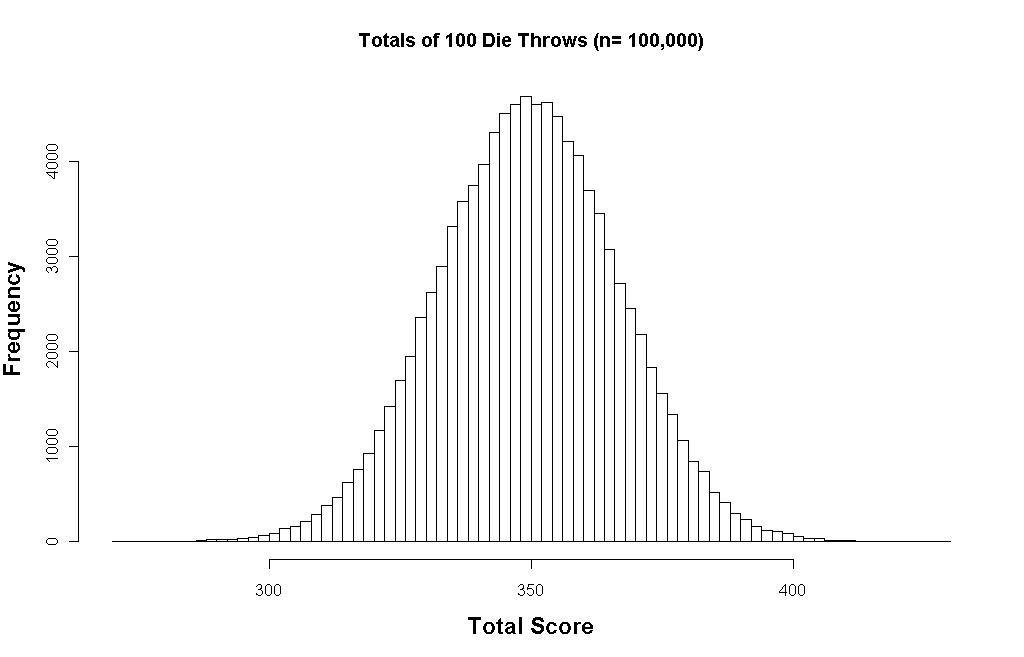
\includegraphics[scale=0.30]{images/3aDieHist3}
		\end{center}
		
		
		
		%=================================================================== %
		
		%\frametitle{Simulation Study}
		A couple of remarks about the simulation study, some of which will be relevant later on.
		\begin{itemize}
			% \item Approximately 76\% of the values are between 330 and 370.
			\item Approximately 68.7\% of the values in the simulation study are between 332 and 367.
			\item Approximately 95\% of the values are between 316 and 383.
			\item $2.5\%$ of the values output are less than 316.
			\item $2.5\%$ of the values study output are greater than 383.
			\item 175 values are greater than or equal to 400, whereas 198 values are less than or equal to 300.
			\item Results such as these are unusual, but they are not impossible.
		\end{itemize}
		
		
		%=================================================================== %
		
		%\frametitle{Random Variables}
		A pair of dice is thrown. Let X denote the minimum of the two numbers which occur.
		Find the distributions and expected value of X.
		
		
		%=================================================================== %
		
		%\frametitle{Random Variables}
		A fair coin is tossed four times.
		Let X denote the longest string of heads.
		Find the distribution and expectation of X.
		
		
		%=================================================================== %
		
		%\frametitle{Random Variables}
		A fair coin is tossed until a head or five tails occurs.
		Find the expected number E of tosses of the coin.
		
		%=================================================================== %
		
		%\frametitle{Random Variables}A coin is weighted so that P(H) = 0.75 and P(T ) = 0.25
		
		The coin is tossed three times. Let X denote the number of
		heads that appear.
		\begin{itemize}
			\item (a) Find the distribution f of X.
			\item (b) Find the expectation E(X).
		\end{itemize}
		
		
		%=================================================================== %
		
		\begin{itemize}
			\item Now consider an experiment with only two outcomes. Independent repeated trials of such an experiment are
			called Bernoulli trials, named after the Swiss mathematician Jacob Bernoulli (1654–1705). \item The term \textbf{\emph{independent
					trials}} means that the outcome of any trial does not depend on the previous outcomes (such as tossing a coin).
			\item We will call one of the outcomes the ``success" and the other outcome the ``failure".
		\end{itemize}
		
		
		%=================================================================== %
		
		\begin{itemize} \item
			Let $p$ denote the probability of success in a Bernoulli trial, and so $q = 1 - p$ is the probability of failure.
			A binomial experiment consists of a fixed number of Bernoulli trials. \item A binomial experiment with $n$ trials and
			probability $p$ of success will be denoted by
			\[B(n, p)\]
		\end{itemize}
		
		%=================================================================== %
 
 MA4004 – Section 1b - Probability Questions
 
 Repeat 2008
 
 Spring 2008
 Question 1
 
 a)   One in 10, 000 people have a particular condition. Given that an individual has this condition, a test for this condition gives a positive result with probability 0.999. Given that an individual does not have this condition, this test gives a positive result with probability 0.001.
 
 Suppose the individual tested is chosen at random from the population as a whole
 i)                  Calculate the probability that the test result is positive.
 
 ii)                Calculate the probability that the individual has the condition, given that the result of the test is positive.
 (6 marks)
 
 Repeats 2007
 
 a) A company obtains 2000 components/week from supplier A, 2000 components/week from supplier B and 1000 components/week from supplier C. 3% of the components from supplier A are defective, 4% of the components from supplier B and 5% of the components from supplier C.
 
 i) Calculate the probability that a randomly chosen component is defective.
 
 ii) Calculate the probability that the component is from supplier A, given that it is not defective.
 (6 marks)
 
 2.              c) Calculate the probability of obtaining exactly 3 sixes when I roll a die
 5 times.
 (4 marks)
 
 
 
 
 
 Spring 2007
 
 a) A company obtains 1500 components/week from supplier A, 1000 components/week from supplier B and 500 components/week from supplier C. 3% of the components from supplier A are defective, 5% of the components from supplier B and 6% of the components from supplier C.
 
 i) Calculate the probability that a randomly chosen component is defective.
 
 ii) Calculate the probability that the component is from supplier C, given that it is defective.
 (6 marks)
 Question 3
 c) Calculate the probability of obtaining exactly 2 sixes when I roll a die 5 times.
 (4 marks)
 
 Repeats 2006
 (c)              A worker-operated machine produces a defective item with probability 0.01 if the worker follows the machine’s operating instructions exactly, and with probability 0.04 if he does not. If the worker follows the instructions 90% of the time, what is the probability that an item produced by the machine, selected at random, will be defective?
 
 
 
\section*{Question 1 : Probability Distribution}

\subsection*{Introduction}{\LARGE Consider playing a game in which you are winning when a \textbf{\emph{fair die}} is showing `six'
	and losing otherwise.}
\subsection*{Part 1}{\LARGE If you play three such games in a row, find the probability mass function (pmf) of the number
	X of times you have won.}

{\LARGE
	\begin{itemize}
		\item Firstly: what type of probability distribution is this?
		
		\item Is this the distribution \textbf{\emph{discrete}} or  \textbf{\emph{continuous}}?
		
		\item The outcomes are whole numbers - so the answer is discrete.
		
		\item So which type of discrete distribution? (We have two to choose from. See first page of formulae)
		
		
		\item \textbf{Binomial:} characterizing the number of \textbf{\emph{successes}} in a series of \textbf{\emph{$n$ independent trials}}, with the \textbf{\emph{probability of a success}} in each trial being $p$.
		
		\item \textbf{Poisson:}  characterizing the \textbf{\emph{number of occurrences}} in a \textbf{\emph{“unit space”}} (i.e. a unit length, unit area or unit volume, or a unit period in time), where $\lambda$ is the the number of occurrences per unit space.
		
	\end{itemize}
}


\subsection{Standardisation Formula}

\begin{equation}
Z = ( X - \mu ) / \sigma
\end{equation}

%----------------------------------------------------------------%

 		\chapter{Discrete Probability Distributions}
Overview
1) The binomial distribution
2) The Poisson distribution
3) 

\section{Poisson Approximation}
The Poisson Approximation of the binomial ditribution

Example

P(X2) = 1- (0.134+0.27) = 0.596

P(X=1) = 2000.010.99199

P(X=1) = 0.270


Poisson Approximaitions


XBinomial(200, 0.01) 


P(X= k)=e-kk!




P(X2) = 1- (0.135+0.27) = 0.595



\section{Probability Formulae}

\begin{itemize}
	
	\item Conditional probability:
	\begin{equation*}
	P(B|A)=\frac{P\left( A\text{ and }B\right) }{P\left( A\right) }.
	\end{equation*}
	
	
	\item Bayes' Theorem:
	\begin{equation*}
	P(B|A)=\frac{P\left(A|B\right) \times P(B) }{P\left( A\right) }.
	\end{equation*}
\end{itemize}
\subsection*{Section 3 : Probability}

How to Compute Probability: Equally Likely Outcomes
Sometimes, a statistical experiment can have n possible outcomes, each of which is equally likely. Suppose a subset of r outcomes are classified as "successful" outcomes.

The probability that the experiment results in a successful outcome (S) is:

P(S) = ( Number of successful outcomes ) / ( Total number of equally likely outcomes ) = r / n

Consider the following experiment. An urn has 10 marbles. Two marbles are red, three are green, and five are blue. If an experimenter randomly selects 1 marble from the urn, what is the probability that it will be green?

In this experiment, there are 10 equally likely outcomes, three of which are green marbles. Therefore, the probability of choosing a green marble is 3/10 or 0.30.

\begin{itemize}
	\item Conditional probability
	\item Independent events
	\item Repeated independent events
\end{itemize}


%------------------------------------------------%
\section{Mutually Exclusive Events}
Mutually exclusive events are events that cannot happen at the same time.
\[ P(A and B) = P(A) + P(B) \]

%------------------------------------------------------------------------------------------------%
%------------------------------------------------------------------------------------------------%
%------------------------------------------------------------------------------------------------%
\section{Quantiles}

The quantile (this term was first used by Kendall, 1940) of a distribution of values is a number xp such that a proportion p of the population values are less than or equal to xp. For example, the .25 quantile (also referred to as the 25th percentile or lower quartile) of a variable is a value (xp) such that $25\%$ (p) of the values of the variable fall below that value.

Similarly, the $0.75$ quantile (also referred to as the 75th percentile or upper quartile) is a value such that $75\%$ of the values of the variable fall below that value and is calculated accordingly.

See



%------------------------------%
\section{Probability Distribution}

A statistical function that describes all the possible values and likelihoods that a random variable can take within a given range. This range will be between the minimum and maximum statistically possible values, but where the possible value is likely to be plotted on the probability distribution depends on a number of factors, including the distributions mean, standard deviation, skewness and kurtosis.



\section{The binomial distribution }

The binomial distribution  is a discrete probability distribution that is applicable as a model for decisionmaking
situations in which a sampling process can be assumed to conform to a Bernoulli process. A Bernoulli
process is a sampling process in which
\begin{itemize}
\item[(1)] Only two mutually exclusive possible outcomes are possible in each trial, or observation. For
convenience these are called success and failure.
\item[(2)] The outcomes in the series of trials, or observations, constitute independent events.
\item[(3)] The probability of success in each trial, denoted by p, remains constant from trial to trial. That is,
the process is stationary.
\end{itemize}

The binomial distribution can be used to determine the probability of obtaining a designated number of
successes in a Bernoulli process. Three values are required: the designated number of successes (X); the number
of trials, or observations (n); and the probability of success in each trial (p). Where $q = (1 - p)$, the formula for
determining the probability of a specific number of successes X for a binomial distribution is

\[ \mbox{Formula} \]


\chapter{Continuous Probability Distributions}
MathsCast 3 : The Uniform Distribution



The Uniform distribution is characterised by two parameters , the minimum and the maximum.

The expected value E(x) is given by



(i.e. the average of the maximum and minimum)





R Code for Graphics

y=c(20,20)
x=c(20,100)

plot(x,y,xlim=c(0,120),ylim=c(0,30),pch=13,col='white',axes=FALSE)
segments(20,20,100,20,col= 'red')
segments(0,0,120,0)

segments(20,0,20,20,col='red')
segments(100,0,100,20,col='red')

segments(0,0,0,40)

\section*{Uniform Distribution: Exercise 24}

Use the uniform distribution to simulate 100 throws of two dice. The outcome is the combined values of both dice. Use the appropriate R command to discretize values.
\begin{itemize}
	\item  What is the mean and standard deviation of the outcomes?
	\item  Make a stem-and-leaf plot of the outcomes.
	\item Make a histogram of the outcomes. (hint: use breaks =seq(1.5,12.5))
\end{itemize}



\subsection{Example 2}
A machine produces components whose thicknesses are normally
distributed with a mean of 0.40 cm and a standard deviation of 0.02 cm.
Components are rejected if they have a thickness outside the range 0.38 cm
to 0.41 cm.
\begin{itemize}
\item[(i)] What is the probability that a component will have a thickness
exceeding 0.41 cm? (4 marks)
\item[(ii)] What is the probability that a component will have a thickness between
0.38 cm and 0.41 cm? (4 marks)
\item[(iii)] What is the thickness below which 25\% of the components will be? (4 marks)
\end{itemize}

\subsection{Example 3}
A charity believes that when it puts out an appeal for charitable donations the
donations it receives will normally distributed with a mean £50 and standard
deviation £6, and it is assumed that donations will be independent of each
other.
\begin{itemize}
	\item[(i)] Find the probability that the first donation it receives will be greater
	than £40.
	\item[(ii)] Find the probability that it will be between £55 and £60.
	\item[(iii)] Find the value x such that 5\% of donations are more than £x.
\end{itemize}


%------------------------------------------------------------------------------------------------%		\section*{Session 09: Probability}
\begin{itemize}
	\item[9B.1] Permutation
	
	\[ {n \choose r} = \frac{n!}{(n-r)! r!} \]
	
	
	\[ {6 \choose 3} = \frac{6!}{(6-3)! 3!} = \frac{6!}{3! \times 3!}\]
	
	
	\[ \frac{6!}{3! \times 3!} = \frac{6 \times 5 \times 4 \times 3!}{3! \times 3!} = \frac{120}{6} = 120\]
\end{itemize}



\begin{itemize}
	\item pairwise disjoint sets
	\item The addition principle
\end{itemize}
\subsection*{Theorem}
\[ |A \cup B| = |A| + |B| - |A \cap B|  \]

\subsection*{Probability}
\begin{itemize}
	\item[9B.2] The sample space of an experiment ($S$)
	\item[9B.3] The size of a sample space
	\item[9B.4] Indepedent Evcents (9.3.1)
\end{itemize}
%------------------------------------------------%

\chapter{Normal Probability Distribution}
MA4004 Revision Class B
Please sign the attendance sheet

Today's class : Last years past paper 


Normal Distribution Question ( Dr David Ramsey's Equine Stats Class)

The mass of Arab horses is normally distributed with mean 900 lbs and standard deviation of 50lbs.
Part i Calculate the probability that an Arab horse weighs more than 940 lbs.


Solution

Let X be mass of Arab horses.

We have to find P(X940).            (Remark "equality component" is included as a formality, but it is not important)


Find the Z value that corresponds to 940 

Zo=Xo-=940 -90050= 0.8

P(X940) = P(Z0.8) 


From Murdoch Barnes tables 3, we find that  P(Z0.8) = 0.2119



Part ii Calculate the probability than an Arab horse weighs between 880 lbs and 960 lbs.
Solution 

P ( 880X960).


What proportion of horses are between 880 lbs and 960 lbs?

Find out the probability of the complement event.
The complement event is the combination of being too high  or too low for this interval.

Inside interval P ( 880X960).

Outside interval P (X880) +P(X960)

Complement Rule P ( 880X960)  = 1 - [P (X880) +P(X960)]



Find the probability of being too high?

Zo=Xo-=960 -90050= 1.2

P(X960) = P(Z1.2) = 0.1151


Find the probability of being too low?
Zo=Xo-=880 -90050= -0.4 
P(X880) = P(Z-0.4)  

How to compute P(Z-0.4)

Symmetry: 	P(Z-0.4) = P(Z0.4) = 0.3446


Outside Interval = 0.4596        (0.3446 +  0.1151)
Inside Interval = 0.5404



What weight is exceeded by 97.5% of Arab horses?

Find Xo  such that P(XXo) = 0.975


P(Z1.96) = 0.025     [From Tables] 

P(Z-1.96) = 0.025  [Symmetry]

P(Z-1.96) = 0.975         

-1.96 =Xo- 90050


Xo= 802 lbs  [Answer]







Question 3 : Hypothesis Testing and Confidence Intervals
Question 4 : Hypothesis Testing and Confidence Intervals

Important:

Formulae at back of Exam Paper
Murdoch Barnes Table 3 (The Z distribution)
Murdoch Barnes Table 7 (The Student t distribution)

Important Considerations

Significance     /    confidence 1-

Number of tails   
one tailed procedure or two tailed procedure
Confidence intervals are always two tailed

Sample size   ( degrees of freedom depends on sample size)




Question 3 - Paired T test

a) The weights of one group of Irish students were recorded both at the beginning of year 1 of their studies and at the end of year 4.
The results (in kg) are given below:

Student
1
2
3
4
5
6
7
8
Year 1
72
58
68
81
65
69
75
84
Year 4
74
61
69
83
69
74
76
82

At a significance level of 5%, is there sufficient evidence to state that on average students gain weight over the four years of their university studies?


Solution

Before we start, we need to compute the average difference and the standard deviations of the differences. 

Student
1
2
3
4
5
6
7
8
Diff
2
3
1
2
4
5
1
-2
Di-D
0
1
-1
0
2
3
-1
-4


Computing the average difference




Now we compute the standard deviation of the variances

From each difference value, subtract the mean, and square the resulting term.


Di-D
0
1
-1
0
2
3
-1
-4
(Di-D)2
0
1
1
0
4
9
1
16





= 4.571

Standard deviation is the square root of the variance

SD=4.571=2.137



hypotheses

H0:D0    Students have not gained weight through college



Ha:D> 0    Students have  gained weight through college


N.B. This is a one-tailed test.

Test statistic

Remember the general structure of a test statistic

TS =Observed Value-Null ValueStd. Error 



Standard Error		S.E.(D) =SDn=2.1378= 0.7555

Test statistis is a t random variable

Test Statistic		x-0S.E.(D)=2 - 00.755= 2.649


Critical values

The sample size (n=8) is small (n30). Use t distribution with n-1 degrees of Freedom.


The test is one tailed.  k= 1  ( ">" symbol in the alternative hypothesis).


Column = k =0.051= 0.05


Murdoch Barnes table 7


Row: df = 7

Column = 0.05

Critical value =  1.895    

Decision rule


Is the test statistic value greater than the critical value?

If Yes: we reject the null hypothesis

If No: We fail to reject the null hypothesis. (not enough evidence)


Here TS = 2.64  is greater than CV = 1.895.


We reject the null hypothesis. Students do put on weight during college. 
Question 3 Part b : Confidence interval for the difference in means of two samples.

b) The mean and standard deviation of the weights of a sample of Irish students according to sex are given below


Number
Mean
Std. Dev.
Male
100
75
10
Female
110
66
8

i)        Calculate a 99% confidence interval for the difference between the mean weight of all male
students and the mean weight of all female students.(7 males)

General Structure of a Confidence Interval





Observed difference

let X denote the weights of male students    X= 75
let Y denote the weights of female students  Y= 66

The difference in the mean of weights X-Y= 9

Quantile

Large sample (both groups are greater than 30).

Population variance is unknown.
Use t distribution with  degrees of Freedom.


Confidence level is 99%. Therefore significance levels is 1%.
Confidence intervals are always two tailed procedures.


Column = k =0.012= 0.005


Murdoch Barnes table 7


Row: df =  
Column = 0.005

Quantile =  2.576 


Stardard Error






Confidence Interval is therefore

99% CI = 9(2.5761.256) 


Part (ii)
Based on this confidence interval, test the hypothesis that on average male students are 6kgs heavier than female students.
State your hypotheses clearly. What is the significance level of this test?   (3 marks)

H0:X-y= 6




Since  we do not reject the null hypothesis at a significance level of 1%.






Question 4

a) The mean and standard deviation of the salaries of 16 Irish full-time workers are €5000  and €3000, respectively.

i)  Test the hypothesis that the mean salary of all Irish full-time workers is €4000 at a significance level of 5%.   (6 marks)



Step 1 : Formally state the null and alternative hypotheses
Step 2 : Determine the test statistic
Step 3 : Determine the critical value
Step 4 : Decision Rule



Given

Observed value : Sample mean     x= 5000 
Null Value (Expected mean under null hypothesis)     o= 4000   
Population standard deviation is unknown.
Use sample standard deviation s = 3000 as an estimate.
Significance  = 0.05
Sample size n = 16  ( small sample)

hypotheses

H0:=4000    True mean salary is €4000
Ha:4000    True mean salary is  not €4000

Test statistic

Remember the general structure of a test statistic

TS =Observed Value-Null ValueStd. Error 



Standard Error		S.E.(x) =sn=300016= 750

Test Statistic		x-0S.E.(X)=5000 -4 000750= 1.33


Critical values

The sample size (n=16) is small (n30). Use t distribution with n-1 degrees of Freedom.


The test is two tailed.  k= 2  ( "" symbol in the alternative hypothesis).


Column = k =0.052= 0.025


Murdoch Barnes table 7


Row: df = 15         (n-1)

Column = 0.025

Critical value =  2.131 


Decision rule


Is the test statistic value greater than the critical value?

If Yes: we reject the null hypothesis

If No: We fail to reject the null hypothesis. (not enough evidence)


Here TS = 1.33  is not greater than CV = 2.131.


We fail to reject the null hypothesis. We can not rightly say that the mean salary is not €4000 per month.


ii)      What assumption is made in this testing procedure? Is this assumption reasonable?  (2 marks)

The assumption made in this testing procedure is that salaries are normally distributed.
This is not a valid assumption as the distribution of salaries is known to be skewed (lots of low values, few high values).







b) A survey of 1000 Irish indicates that 750 have access to the Internet. A survey of 2000 Spaniards indicates that 1400 have access to the Internet.

i)        By calculating the appropriate p-value, test the hypothesis that the proportion of all Irish having access to the Internet
is equal to the proportion of all Spaniards having access to the internet at a significance level of 5%. (8 marks)


Step 1 : Formally state the null and alternative hypotheses

Step 2 : Determine the test statistic
Step 3a : Determine the p.value
Step 4a : Decision Rule for p-values.



Step 1 : Formally state the null and alternative hypotheses

Proportion of people having internet access is the same in both Ireland and Spain
Proportion of people having internet access differs in Ireland and Spain


Alternatively we write the hypotheses as follows (the null value is more evident).





Step 2 Compute the Test Statistic

pIrl=7501000= 0.75 
pEsp=14002000= 0.70

Observed Difference = 0.75 - 0.70 = 0.05  

Now lets compute the standard error (from Formulae)


ii)      Calculate a 99% confidence interval for the difference between the proportion of all Irish having access to the
Internet and the proportion of all Spaniards having access to the internet.  (4 marks)
]

Standard Error for confidence interval	p1(1 -p1)n1+p2(1 -p2)n2	=0.750.251000+0.700.302000     =  0.017103



Quantile for a 99% confidence interval

significance level  =1%
number of tails = 2
degrees of freedom = 
quantile = 2.576 


99% Confidence Interval for difference of two proportions












Useful pieces of information


Sample size  n=100




Part i
Calculate the equation of the least square regression line and interpret the value of the slope.
part ii

Using this regression model, estimate the mean weight of individuals who are 3 metres tall.
part iii

Is such an estimate reliable?  briefly explain why.

No it is not reliable. Consider the range of values of the x predcitro variable










\section{Normal Distribution: Worked Examples}

% % MA4413    Computer Maths 3     January 2007


Q5. a) Assume that the amount of wine poured into a bottle has a normal distribution with a mean of 750ml and a variance of 144ml$^2$.

\begin{itemize}

\item[(i)]  Calculate the probability that a bottle contains more than 765ml. (2 marks)
\item[(ii)]    Calculate the probability that a bottle contains between 744ml and 759ml. (3 marks)
\end{itemize}
%=========================================================== %
A machine fills bags with animal feed. The nominal weight of a bag is 50kg.
Because random variations the weight of a filled bag is normally distributed
$N(\mu, \sigma^2)$. The variance ($\sigma^2$) is known to be 0.01kg$^2$ and $\mu$ is set by the
operator to a particular value.

(i) If ? = 50kg calculate the probability of a bag containing less than
49.95kg?
(ii) Calculate the value of "?" such that only $2\%$ of the output are under the
nominal weight?



MA4004     Engineering Statistics    SPRING 2008


a)	The amount of beer in a bottle has a normal distribution with mean 500ml and variance 25ml2.
i)	Calculate the probability that the amount of beer in the bottle is between 498ml and 504ml.
ii)	What volume is exceeded by $20\%$ of the bottles?
(6 marks)

%--------------------------------------------------------------------------------------%




%---------------------------------%

\subsection{The Standard Normal Distribution}



\section*{Session 09: Probability}
	
		\begin{itemize}
			\item pairwise disjoint sets
			\item The addition principle
		\end{itemize}
		\subsection*{Theorem}
		\[ |A \cup B| = |A| + |B| - |A \cap B|  \]
		
		\subsection*{Probability}
		\begin{itemize}
			\item[9B.2] The sample space of an experiment ($S$)
			\item[9B.3] The size of a sample space
			\item[9B.4] Indepedent Evcents (9.3.1)
		\end{itemize}
		%------------------------------------------------%
		\section*{Session 9 Probability}

		

\section{Discrete Random Variables}
	%----------------------------------------------------------%
	\begin{enumerate}
		\item  The probability distribution of discrete random variable $X$ is tabulated below. There are 6 possible outcome of $X$, i.e. 0, 1, 2, 4 ,8 and 10.
		\begin{center}
			\begin{tabular}{|c||c|c|c|c|c|c|}
				\hline
				$x_i$  & 0 & 1 & 2 & 4 & 8 & 10 \\\hline
				$P(x_i)$ & 0.25 & 0.15 & 0.25 & 0.15 & k & 0.10\\
				\hline
			\end{tabular}
		\end{center}
		
		\begin{itemize}
			\item[i.] (1 marks) Compute the value for $k$.
			\item[ii.] (3 marks) Determine the expected value $E(X)$.
			\item[iii.] (2 marks) Evaluate $E(X^2)$.
			\item[iv.] (3 marks) Compute the variance of random variable $X$.
		\end{itemize}
		%---------------------------------------------------------- %
		%Question 2
		\item 
		Suppose $X$ is a random variable with 
		\begin{itemize}
			\item $E(X^2)=3.6$
			\item $P(X=2)=0.6$
			\item $P(X=3)=0.1$
		\end{itemize}
		
		\begin{itemize}
			\item[(a)] The random variable takes just one other value besides 2 and 3. This value is greater than 0. What is this value?
			\item[(b)] What is the variance of $X$?
		\end{itemize}
		
		
		%Question 6
		\item Consider the random variables $X$ and $Y$. Both $X$ and $Y$ take the values 0,$\;$1 and 2. 
		The joint probabilities for each pair are given by the following table.
		\begin{center}
			\begin{tabular}{|c|c|c|c|}
				\hline  & $X=0$ & $X=1$ & $X=2$ \\ 
				\hline $Y=0$ & 0.1 & 0.15 & 0.1 \\ 
				\hline $Y=1$ & 0.1 & 0.1 & 0.1 \\ 
				\hline $Y=2$ & 0.2 & 0.05 & 0.1 \\ 
				\hline 
			\end{tabular} 
		\end{center}
		Compute the $E(U)$ expected value of $U$, where $U=X-Y$.
	\end{enumerate}
	\newpage
	{\Large
		\begin{itemize}
			
			\item Suppose we have a set of \textbf{n} items.
			\item From that set, we create a subset of \textbf{k} items.
			\item The \textbf{order} in which items are selected is recorded. (The ordering of selected items is very important.) 
			\item The total number of \textbf{ordered subsets} of \textbf{k} items chosen from a set of \textbf{n} items is
			
			\[\frac{n!}{n-k!}\]
		\end{itemize}
	}
	%----------------------------------------------------------------------------------------------------%
	
	
	An ordered sequence of four digits is formed by choosing digits without
	repetition from the set $\{1, 2, 3, 4, 5, 6, 7\}$ .
	
	\begin{itemize}
		\item[(i)] the total number of such sequences; (780)
		\item[(ii)] the number of sequences which begin with an odd number; (480) N(A)
		\item[(iii)] the number of sequences which end with an odd number; (480) (NB)
		\item[(iv)] the number of sequences which begin and end with an odd number;(240)
		\item[(v)] the number of sequneces which begin with an odd number or end with an
		odd number or both; (720)
		\item[(vi)] the number of sequences which begin with an odd number or end with an
		odd number but not both. (480)
	\end{itemize}
	
	%----------------------------------------------------------------------------------------------------%
	
	
	A college teaches a range of courses including maths, physics and IT.
	Students choose a range of courses from these three subject areas. Currently 600
	students are enrolled of whom 300 study maths courses, 120 study IT
	and 380 study physics courses. 
	
	\begin{itemize}
		\item 40 students study courses from all three subject
		areas. 
		\item 200 maths students study physics as well. 60 physics students
		also study IT and 70 IT students also study maths. 20 students study physics and IT, but not maths.
	\end{itemize}
	
	
	%----------------------------------------------------------------------------------------------------%
	
	\begin{itemize}
		\item How many students study none of these courses at all? (90)
		
		\item How many students study maths but not physics or IT? (70)
		
		\item How many students study both maths and physics but not IT? (160)
		
		\item How many students study courses from precisely two of these subject
		areas? (210)
	\end{itemize}
	
	%----------------------------------------------------------------------------------------------------%
	
\end{document}
